\newif\ifdraft\draftfalse
\newif\iflinenumbers\linenumberstrue
\newif\ifnomenclature\nomenclaturefalse
\newif\ifnotes\notestrue
\newif\ifendfloat\endfloatfalse

% Draft commands --------------------------------------------------------------
\ifdraft
  \documentclass[12pt,number,preprint,review,times]{elsarticle}
  \ifendfloat
    \usepackage[markers]{endfloat}
    \renewcommand{\efloatseparator}{\mbox{}}
  \fi
  \iflinenumbers
    \usepackage[modulo]{lineno}
    \renewcommand\linenumberfont{\ttfamily\upshape\footnotesize}
  \fi
  \usepackage{geometry}
  \geometry{a4paper,top=2cm,bottom=2cm,left=3cm,right=3cm}

% Final version ---------------------------------------------------------------
\else
  \documentclass[10pt,number,final,5p,times,twocolumn]{elsarticle}
  \notesfalse
  \linenumbersfalse
  \endfloatfalse
\fi
\setlength {\marginparwidth }{2cm}
% General packages ------------------------------------------------------------
\usepackage[T1]{fontenc}
\usepackage[utf8]{inputenc}
\usepackage[fleqn]{amsmath}
\usepackage{amssymb}
\usepackage{bm}
\usepackage{nextpage}
\usepackage{setspace}
\usepackage[mode=buildnew]{standalone}
\usepackage{xcolor,todonotes}
\usepackage[normalem]{ulem}
\usepackage[colorlinks=true]{hyperref}
\usepackage{caption}
\usepackage{subcaption}
\captionsetup{font=normalsize}
% \usepackage{siunitx}
% \sisetup{output-exponent-marker=\ensuremath{\mathrm{e}}}
% Graphics --------------------------------------------------------------------
\usepackage{graphicx}
\graphicspath{{./}}
\usepackage{tikz}
%\usepackage{gnuplot-lua-tikz}

\usetikzlibrary{shapes,arrows}

% Tables ----------------------------------------------------------------------
\usepackage{booktabs}
\usepackage{multirow}

% Number format ---------------------------------------------------------------

\usepackage[autolanguage,np,nosepfour]{numprint}

\usepackage{siunitx}
\sisetup{
  mode=math, % text | math
  exponent-product = \cdot,
  math-rm = \ensuremath,
  round-mode = off, % off | figures | places
  scientific-notation = false, % true | false | engineering
  output-decimal-marker = {.},
  retain-zero-exponent = true,
  separate-uncertainty = true,
  %multi-part-units = repeat,
  % round-integer-to-decimal = true,
  round-precision = 2,
}

  

% References ------------------------------------------------------------------
\usepackage[noabbrev]{cleveref}

% Bibliography ----------------------------------------------------------------
\usepackage{natbib}
% \bibliographystyle{elsarticle-num-names}
\bibliographystyle{optplainnat}
\biboptions{sort&compress}

% Nomenclature ----------------------------------------------------------------
\ifnomenclature
  \usepackage{nomencl}
  \makenomenclature
  \renewcommand{\nomlabelwidth}{2.2cm}
\else
  \usepackage{nomencl}
\fi

\begin{document}

% \newpage

\begin{frontmatter}
\title{Analytical and numerical crashworthiness uncertainty quantification of metallic thin-walled  energy absorbers}

% \title{On the uncertainty/error of analytical and semi-empirical approximations of mean and peak crushing force of energy absorbers}

% \title{Uncertainty quantification of analytical and semi-empirical approximations of mean and peak crushing force of energy absorbers}


\author{
J. Paz \footnote{PostDoc researcher. Corresponding author. Tel: +34 881 016 017; Fax: +34 981 167 170},
J. D\'{\i}az\footnote{Associate Professor},
L. Romera\footnote{Associate Professor}, \\
{\normalsize\itshape
Universidade da Coru\~{n}a -- Structural Mechanics Group, School of Civil Engineering} \\ 
{\normalsize\itshape 15071 A Coru\~{n}a, Spain }}

\begin{abstract}

This research focuses on the crashworthiness uncertainty quantification of thin-walled tubes under axial loads. The error propagation of the two cross-sections studied, circular and square, is performed for numerical, geometrical, material, and impact uncertainties. Three methods are used: a statistical error propagation of the analytical formulas, the UQ from a surrogate model from the formulas, and from a surrogate model built from finite element simulations. Results show that the best approximation is offered from the MARS metamodel, yielding similar mean values as with statistical propagation and a standard deviation overshot by 1\% to 3\%. The numerical numerical noise quantified for the simulations results in oscillation frequencies below 40\% and a breadth of three-sigma below 9\% for both metrics. The UQ of both tubes offers similar results when studying geometric uncertainties, although the opposite is found if material uncertainties are considered. Uncertainties in the impact conditions lead to reduced peak load values when the impact angle varies from a perfect axial collision, consequently delivering reduced  mean  values  and  high  standard deviations.
 
 
\end{abstract}

\begin{keyword}
Crashworthiness \sep Uncertainty quantification \sep crushable energy absorbers
\end{keyword}

\journal{Thin-walled Structures}

\end{frontmatter}

% \tableofcontents

% \listoffigures
 
% \listoftables

\section{Introduction}
 
% -Crashworthiness uncertainty quantification of energy absorption tubes for robust design.

% -UQ Tubes

% -UQ Numerical noise / Effect of shell elements / Surrogate model uncertainty

% -UQ Impact conditions

% -Dakota capabilities

% \begin{itemize}
%     \item UQ analytical from TWT formulas
%     \item UQ surrogate from TWT formulas
%     \item UQ surrogate from FEA
% \end{itemize}

Amid the main research lines for the enhancement of aircraft and automotive designs, structural optimization and crashworthiness studies are at their pinnacle. Means of transport need to be robust and safe, albeit efficiency and lightness cannot be neglected. While active safety systems have avoided innumerable accidents, passive crashworthiness systems need to protect passengers when they do occur. In the event of a crash, modern structures are designed to collapse progressively, dissipating high amounts of kinetic energy and protecting the passengers against abrupt decelerations. 

Thin-walled crushable tubular structures are among the most common energy absorption devices used by the transport industries. They can be featured as structural elements in aircraft and helicopter subfloor structures \citep{Paz2019IJCW,Paz2020,bisagni2002crashworthiness}, front deformation areas for cars \citep{White1999179,White1999209} or trains \citep{marsolek2004energy}, and even as roll-over protection structures on construction machinery \citep{ahmad2009application}. As \citet{alghamdi2001collapsible} identified, collapsible energy absorbers' shape and thickness-to-weight ratios are similar independently of the scale difference between aircraft, automobile or train structures. Their energy dissipation profile is influenced by many factors, as the magnitude and application of the load, the strain-rate sensitivity of the materials or the deformation mode occurring \citep{johnson1978metallic}. 

The ultimate goal in using collapsible energy absorbers is that of converting the highest amount of kinetic energy into another form of energy \citep{stronge2004impact}. Crushable tubes dissipate kinetic energy through plastic deformation, which can unfold under several modes depending on their cross-section shape, load diES
rection, and the ratios between cross-sectional inertia, length, and wall thickness \citep{lu2003energy}. The first studies on collapsible tubes are attributed to J. M. \citet{Alexander}, after obtaining the approximate theoretical expression of the mean axial crushing force in thin-walled circular tubes back in the 1960s. Almost 20 years later, \citet{wierzbicki1983crushing} developed the super folding element theory which investigated theoretical predictions for the axial mean crushing strength of rectangular tubes. In the experimental models from \citet{abramowicz1989axial}, \citet{abramowicz1986dynamic}, \citet{Pugsley19791}, and \citet{Singace19963517}; Alexander's tube was redesigned by shaping it with rectangular, circular and multi-corner sections; which was later axially crushed, loaded both statically and dynamically. They also carried out multiple studies dealing with the different collapse modes, obtaining a sensible resemblance between the theoretical predictions and the experimental results \citep{Abramowicz1997415}.

Axial crushing is the most common energy dissipating method, primarily due to its high capabilities as an energy dissipation device \citep{sadeghi1984design}. When compared to other deformation modes, energy dissipation values can be up to ten times higher for the same tube, as proved by \citet{reid1985metal}. Axial crushing in tubes can develop under three different modes, with the progressive crushing being inherent of metallic specimens; and the splaying and fragmentation mechanisms characteristic of those made from composites \citep{hull1991unified}. Moreover, progressive folding is further subdivided according to the collapse evolution; which is in turn determined by the geometry of the absorber and the load conditions. \citet{andrews1983classification} classified the progressive crushing of circular tubes under quasi-static loading into three categories, of which the concertina and diamond modes of deformation are the most recurrent. The concertina mode is axisymmetric and typical of tube with diameter-to-thickness ratios under 50 \citep{guillow2001quasi}. Diamond collapse modes are non-axisymmetric and exhibit specific energy absorption values slightly lower than in the concertina mode \citep{andrews1983classification}. This mode occurs when the diameter-to-thickness ratio is over a hundred, with mixed collapse modes in the 50 to 100 range. \citet{wang2002mushrooming} described a fourth plastic deformation mode for impact speeds over \num{100} m/s, named ``mushrooming'' honoring the post-test shape resulting. Square-section thin-walled tubes experience different collapse modes than their circular relatives, although force-displacement trends are similar when undergoing progressive crushing.


Another method for the prediction of the crush behaviour of thin-walled tubes resides in the use of computational models and finite element analyses (FEAs). FEAs are considered first-principles or fully predictive methods, so with the correct characterization of the model's shape, material and simulation conditions, results accurately mimic the experimental process without previous adjustment required \citep{noor1993computational}. Moreover, the evaluation of structures through numerical simulations not only translates into less expenses, but also allows assessing a wider range of models and impact conditions, many of which may not be experimentally tested. The detailed crush behavior and energy dissipated by the components can be effortlessly retrieved, data not so easily obtained from experimental methods \citep{altenhof2002experimental}.




% Thin-walled structural members 
However, and despite the many advancements implemented in FEA to improve simulation's computational time, robustness, and accuracy, certain shortcomings as noise and repeatability still affect the fidelity of non-linear dynamic analyses \citep{zhu2013lightweight}. Of particular interest is the quantification of numerical noise in CFD simulations performed by \citet{gilkeson_dealing_2014}, decomposing the oscillation into frequency and amplitude. A sensitivity study was also performed considering the impact of the grid type, cell type, and turbulence model; which for our particular case of study will analogously translate into determining the effect of using different mesh sizes. Moreover, the explicit time step scheme, memory parallelization, and contact formulation used in such non-linear simulations lead to results not often repeatable \citep{jeong2010non}, which may even trigger the extreme example of bifurcation where unique structural reaction patterns appear \citep{will_robustness_2006,duddeck_multidisciplinary_2008}.

During deterministic design and optimization processes, no room is left for the consideration of the uncertainties involved in real-life engineering problems, which may comprise the aforementioned numerical noise, loading conditions, material properties, geometries, or manufacturing tolerances. One tool for the design of robust structures is that of parameter screening and selection, where the effect of varying the design parameters along their feasible domain is assessed to determine which have the largest influence on the monitored metrics \citep{giannini_case_nodate,gao_sensitivity_2019}. Moreover, uncertainty quantifications (UQ) methods propagate these incertitudes to the objective metrics, obtaining a probabilistic function with its own statistical moments \citep{fang2017design}. 

Deepening into the diversity of uncertainty variables used in crashworthiness applications, impact conditions are commonly considered in UQ analyses, as impact angle and velocity can severely influence the component's structural response \citep{ren_crashworthiness_2014}. Geometry effects are also typically studied, with authors as \citet{eichmueller_computer_2019} proving that slight thickness variations in an axially-loaded square tube can cause relevant dispersion of the component's behavior both at low and high testing speeds. Material uncertainties as the elastic and tangential moduli, Poisson's ratio, density, or the yield stress can also be considered to account for the discrepancies induced by the manufacturing process between the nominal design and the resulting real product \citep{sun2011crashworthiness,najafi2014multi}. % The usage of triggers is also studied given their effect on the global collapse process of the tubes and their crashworthiness response \citep{Paz2015499}.

Surrogate models are an efficient tool for characterizing such numerical stochastic phenomena, reducing computational costs during UQ and, specially, when seeking RBDO \citep{moustapha_adaptive_2015}. However, the main issue with the use a surrogate model is its accuracy, as substituting the real responses by a a numerical model may also introduce metamodeling uncertainty to the results \citep{zhang_concurrent_2013,qiu_crashworthiness_2018}. Two of the most commonly used regression metamodels are polynomial response surfaces (PRS), which filter most of the numerical noise from the non-linear simulations as those at hand \citep{papila2000response}, and Gaussian processes, where the approximation goes through all the sampling points. With the aim of obtaining reliable results, other surrogate models are also fitted and studied, seeking a conservative surrogate model that helps achieve feasible optimum designs \citep{pan_application_2013} for future phases of this research. 

Rather than jumping directly into reliability analysis and RBDO, this paper will first investigate the stochastic nature of the energy absorption components' behavior due to uncertainties in structural dimensions, material properties, initial impact conditions, and the numerical simulation. This research will attempt to combine the uncertainty quantification approaches and techniques from previous works, later applying this to determine the crashworthiness response of energy absorption tubes under impact scenarios. 

In a first approach, the analytical uncertainty propagation of the most representative analytical formulas is addressed for the two selected tube geometries used, namely square and circular. Realistic values are used for the design variables' statistical parameters, quantifying the robustness of the components under different uncertainty conditions, which include impact velocity, material properties, and geometry. These variables are also screened and ranked according to their influence on the final crashworthiness response. 

Later, the UQ process is repeated numerically for the analytical formulas by coupling them with the metamodelling code. A Latin hypercube sampling is performed over the design space as to fit and compare different surrogate models: polynomial response surfaces, moving least squares, multivariate adaptive regression splines (MARS), and Gaussian process (Kriging). The fitness of the metamodels is assessed according to statistical metrics, determining that most compliant with the analytical results previously obtained. 

The final step in the investigation substitutes the analytical formulas by FE simulations for the sampling and construction of the surrogate model. In this phase, the numerical noise inherent to the simulations is quantified and included as part of the uncertainties considered in the design process. The statistical results from the studied metrics are compared to the results previously obtained as to determine the inaccuracies yielded by the FEAs. This work is a crucial step towards the robust design of energy absorbing components for aircraft and automobile applications through reliability analysis and reliability-based design optimization. %, which will be addressed in subsequent publications.

\section{Analytical models}
\label{sec:intro}
The first phase of this research focuses on the analytical characterization and uncertainty quantification of circular and square thin-walled tubes under axial loading. A baseline model is selected for each geometry, and both are made with the AA2024-T3 aluminum alloy detailed in \cref{tab:alum}. This table also contains the expected value and standard deviation values for the two uncertain variables, the Young's modulus $E$ and the energy equivalent flow stress $\sigma_0$, with the three different coefficients of variation (COV) considered.

\begin{table}[!htpb]
\begin{center}
\small
\begin{tabular}[t]{lrrrr} \toprule
 &  &  \multicolumn{3}{c}{Standard deviation}  \\\cmidrule{3-5}
Parameter & Mean       &    COV = 2 \%  &  COV = 5 \%      &    COV = 10 \%  \\\midrule
E (GPa)  &  73.10 &  1.462 & 3.655 & 7.310   \\
$\sigma_0$ (MPa) &  280.00 & 5.60 & 14.00 & 28.00 \\ %\midrule
$E_t$ (GPa)  &  60.00 &  - & - & -   \\
$\nu$  &  0.33 & - & - & - \\
$\rho$ ($\mathrm{kg/m^3}$) & 2700.00  & - & - & - \\
\bottomrule
\end{tabular}
\captionsetup{justification=centering}
\caption{Properties of AA2024-T3 aluminum alloy \citep{kay2003failure} and statistical parameters. Three different coefficients of variation are considered for the variables.}
\label{tab:alum}
\end{center}
\end{table}

\subsection{Notation}

The notation for the functions studied, $P^{\mathrm{}}_{\mathrm{mean}}$ and $P^{\mathrm{}}_{\mathrm{max}}$, has been selected to particularize each tube shape, source of the result, and the metric in question. The notation takes the form $P^{x}_{{y{\text -}z}}$ where $x$ can be `emp' for the empirical analytical formula, `theo' for the theoretical analytical formula, or `FEA' if stemming from numerical simulations. The tube shape is defined by $y$, where `c' and `s' stand for circular and square cross-sections respectively. Finally, $z$ indicates the metric studied, with `mean' relating to the average crushing force and `max' to the peak force. As for statistic-related notation, $E[\,]$ is used to denote the expected value, $V[\,]$ refers to the variance, and $\sigma[\,]$ is the standard deviation.

\subsection{Circular tube}

The circular tube geometry is defined by a diameter of $D = 80$ mm and a plate thickness of $t_\mathrm{c} = 2$ mm, resulting in a $D/t_\mathrm{c}$ ratio of 40 which ensures the tube's collapse under the concertina mode \citep{guillow2001quasi}. The design variables are assumed to behave according to a normal distribution, with their statistical moments defined in \cref{tab:vars_circ}. Three different coefficients of variance are used for each of the variables.

\begin{table}[!htpb]
\begin{center}
\small
\begin{tabular}[t]{lrrrr} \toprule
\multicolumn{1}{c}{Design} &  &  \multicolumn{3}{c}{Standard deviation}  \\\cmidrule{3-5}
\multicolumn{1}{c}{variable} & Mean       &    COV = 2 \%  &  COV = 5 \%      &    COV = 10 \%  \\\midrule
$D$ (mm) &  80.00 &  1.60 & 4.00 & 8.00   \\
$t_\mathrm{c}$ (mm) &  2.00 & 0.04 & 0.10 & 0.20 \\ %\midrule
% $\nu$  &  0.33 & - & - & - \\
% $\rho$ $\mathrm{kg/m^3}$ & 2700  & - & - & - \\
\bottomrule
\end{tabular}
\captionsetup{justification=centering}
\caption{Statistical moments for the geometrical design parameters of the circular tube. Three different coefficients of variation are considered for the variables.}
\label{tab:vars_circ}
\end{center}
\end{table}

Two analytical formulas are chosen for the prediction of their average crushing force, $P_{\mathrm{c{\text -}mean}}$, and one for the peak crushing force $P_{\mathrm{c{\text -}max}}$. The empirical formula from \citet{guillow2001quasi} estimates $P_{\mathrm{c{\text -}mean}}$ as

\begin{equation}
\centering
    P^{\mathrm{emp}}_{\mathrm{c{\text -}mean}} = 72.3 (D / t_\mathrm{c})^{0.32} M_0,
\label{eq:pmean_emp}
\end{equation}
with $M_0$ being the fully plastic bending moment based on the flow stress, defined as $M_0 = \sigma_{0} \; {t_\mathrm{c}}^2 / {4}$. \citet{Abramowicz1986}, focusing on the theoretical energy dissipation from plastic hinge formation, predicts the average force by

\begin{equation}
\centering
    P^{\mathrm{theo}}_{\mathrm{c{\text -}mean}} = \frac{25.23\sqrt{D/t_\mathrm{c}}+15.09}{0.86-0.568\sqrt{t_\mathrm{c}/D}}M_0
\label{eq:pmean_theo}
\end{equation}

On the other hand, $P_{\mathrm{c{\text -}max}}$ is estimated with the formulas from \citet{plantema1964collapsing}:

% \begin{equation}
% \small
\begin{align}
% \centering
P_{\mathrm{c{\text -}max}} &= \sigma_0 \; {A^c_{\mathrm{S}}}&& \quad \mathrm{for} \quad \alpha \geq 8 \label{eq:pmax1}\\ 
P_{\mathrm{c{\text -}max}} &= (0.75 + 0.031 \alpha) \; \sigma_0 \; {A^c_{\mathrm{S}}}&& \quad \mathrm{for} \quad 2.5 \leq \alpha < 8 \label{eq:pmax2}\\ 
P_{\mathrm{c{\text -}max}} &=  0.3 \; \alpha  \; \sigma_0 \; {A^c_{\mathrm{S}}}&& \quad \mathrm{for} \quad \alpha < 2.5
\label{eq:pmax3}
\end{align}
where ${A^c_{\mathrm{S}}} =  \pi D \, t_\mathrm{c} $ is the cross-sectional area and $\alpha$ is calculated as:
\begin{equation}
\alpha = \frac{E \; t_\mathrm{c}}{\sigma_0 \; D}
\end{equation}

For the studied circular tube, $\alpha \approx 6$, thus using \cref{eq:pmax2} to calculate the analytical $P_{\mathrm{c{\text -}max}}$.

% \end{equation}

To quantify the effect of uncertainties in the design variables, the analytical error propagation of these formulas is performed using the approximations from \citet{hendeby2007nonlinear}. The resulting formulas are hereunder presented, while the integration process to reach them is detailed in \cref{sec:app1}.

Finally, two dimensionless ratios introduced by \citet{pugsley1960crumpling} are studied to assess the efficiency of the thin-walled structures, the structural effectiveness $\eta$ and the solitidy ratio $\phi$. The solidity ratio, also called relative density, is the ratio between cross-sectional area ${A_{\mathrm{S}}}$ and wall cross-sectional area $A_\mathrm{C}$, calculated for the circular tube as: 

\begin{equation}
\phi^c = \frac{A^c_{\mathrm{S}}}{A^c_\mathrm{C}} = \frac{4 t_\mathrm{c}}{D}
\end{equation}
while the structural effectiveness for the circular tube can be obtained from the theoretical formula as
\begin{equation}
\eta_{\mathrm{theo}}^c = \frac{P_{\mathrm{c{\text -}mean}}}{\pi D t_\mathrm{c} \sigma_0 } = \sqrt{ \frac{\pi \phi}{2 \sqrt{3}}  }
\end{equation}
and from the empirical formula from \citet{thornton1983energy}

\begin{equation}
\eta_{\mathrm{emp}}^c = 2 {\left(\phi^c\right)}^{0.7}
\end{equation}
% Analytical formulas and statistical formulas. Integrals in appendix
Particularized for the selected geometry, this coefficients take the values of

\begin{align}
% \centering
\phi^c &= 0.1\\ 
\eta_{\mathrm{theo}}^c &= 0.301\\ 
\eta_{\mathrm{emp}}^c &=  0.399
\end{align}

\subsection{Square tube}

The geometry of the square-sectioned tube is also characterized with two design variables, namely the edge length $C$ and the material thickness $t_\mathrm{s}$. These values have been chosen so that both the circular and square tubes have the same values of cross-sectional area and wall cross-sectional area. This entails choosing a wall thickness $t_\mathrm{s} = \sqrt{\pi} \: t_\mathrm{c} / 2$ and an edge length $C = \sqrt{\pi} \: D / 2$, leading to a square tube with $C=70.90$ mm and $t_\mathrm{s} = 1.77$ mm as the baseline design. \Cref{tab:vars_sq} offers the statistical moments considered for the variables studied.

\begin{table}[!htpb]
\begin{center}
\small
\begin{tabular}[t]{lrrrr} \toprule
\multicolumn{1}{c}{Design} &  &  \multicolumn{3}{c}{Standard deviation}  \\\cmidrule{3-5}
\multicolumn{1}{c}{variable} & Mean       &   COV = 2 \%  &  COV = 5 \%      &    COV = 10 \%  \\\midrule
$C$ (mm) &  70.90 &  1.418 & 3.545 & 7.090   \\
$t_\mathrm{s}$ (mm) &  1.77 & 0.0354 & 0.0885 & 0.177 \\ %\midrule
% $\nu$  &  0.33 & - & - & - \\
% $\rho$ $\mathrm{kg/m^3}$ & 2700  & - & - & - \\
\bottomrule
\end{tabular}
\captionsetup{justification=centering}
\caption{Statistical moments for the geometrical design parameters for the square tube. Three different COV are considered for the variables.}
\label{tab:vars_sq}
\end{center}
\end{table}

To study the crashworthiness response of the tube, two formulas are used to estimate the average crushing force $P_{\mathrm{s{\text -}mean}}$ and one for the peak force $P_{\mathrm{s{\text -}max}}$. The empirical formula from \citet{Abramowicz1984179} predicts $P_{\mathrm{s{\text -}mean}}$ as:

\begin{equation}
\centering
    P^{\mathrm{emp}}_{\mathrm{s{\text -}mean}} = 38.12 (C / t_\mathrm{s})^{1/3} M_0.
\label{eq:pmean_emp_sq}
\end{equation}

Moreover, the effective crushing distance of the tube shall be taking into account into \cref{eq:pmean_emp_sq} following the approach from \citet{Wlodzimier-1983}. For this particular baseline design it is found that this effective crushing distance is approximately 0.85, thus the resulting empirical formula for predicting the average crushing force reads

\begin{equation}
\centering
    P^{\mathrm{emp}}_{\mathrm{s{\text -}mean}} = 44.85 (C / t_\mathrm{s})^{1/3} M_0.
\label{eq:pmean_emp_sq2}
\end{equation}

\citet{wierzbicki1983crushing} have also provided a theoretical formula for the average crushing force of polygonal tubes, reading

\begin{equation}
\centering
    P^{\mathrm{theo}}_{\mathrm{s{\text -}mean}} =  \frac{3 n}{s} \sqrt[3]{2 \pi \, I_{1}(\psi_0) I_{3}(\psi_0)} \; \sigma_0 \, t_\mathrm{s}^{5/3} \, C^{1/3} % \frac{25.23\sqrt{D/t_\mathrm{c}}+15.09}{0.86-0.568\sqrt{t_\mathrm{c}/D}}M_0
\label{eq:pmean_theo_sq}
\end{equation}
where $n$ is the number of corners, $\psi_0$ is the angle between corners ($\psi_0 = \pi / 4$ for the square tube), and  $I_{i}$ are coefficients particularized for each geometry. In the case of square sections, $I_{1}(\pi / 4) = 0.58$ and $I_{3}(\pi / 4) = 1.15$.

On the other hand, the peak crushing force is predicted through \citet{timoshenko2009theory} as:

\begin{equation}
\centering
    P_{\mathrm{s{\text -}max}} = \left[ k \frac{\pi^2 \, E_r}{12 (1 - \nu_r^2)} {\left( {\frac{t_\mathrm{s}}{C}} \right)}^2  + \sigma_{\mathrm{c}} \right] {A^s_{\mathrm{S}}} \; , %  \sqrt[3]{2 \pi \, I_{1}(\psi_0) I_{3}(\psi_0)} \; \sigma_0 \, t_\mathrm{s}^{5/3} \, C^{1/3} % \frac{25.23\sqrt{D/t_\mathrm{c}}+15.09}{0.86-0.568\sqrt{t_\mathrm{c}/D}}M_0
\label{eq:pmax_theo_sq}
\end{equation}
where $k$ is the buckling coefficient taking the value of $k = 6.98$ for the considered boundary conditions, $\sigma_c$ is calculated by
\begin{equation}
\centering
    \sigma_{\mathrm{c}} = \sigma_{\mathrm{y}} \left[ 1 - \left( {\frac{E_r}{E}} \right) \left( {\frac{1 - \nu^2}{1 - \nu_r^2}} \right) \right], 
\label{eq:pmax_sigma-c}
\end{equation}
with $\sigma_{\mathrm{y}}$ representing the material's yield stress, $E_r$ being defined by 
\begin{equation}
\centering
    E_r = \frac{4 E E_t}{\left( \sqrt{E} + \sqrt{E_t} \right)^2} \; , 
\label{eq:pmax_Er}
\end{equation}
$E_t = {\partial \sigma}/{\partial \varepsilon}$ being the tangent modulus, and $\nu_r = 0.5$.


The solitidy ratio and structural effectiveness are also quantified for the square tube, with the former being

\begin{equation}
\phi^s = \frac{{A^s_{\mathrm{S}}}}{A_\mathrm{C}} = \frac{4 t_\mathrm{s}}{C},
\end{equation}
while \cref{eq:pmean_emp_sq2} can be transformed into 
\begin{equation}
\eta_{\mathrm{theo}}^s = 1.11 {\left(\phi^s\right)}^{2/3}.
\end{equation}

\citet{thornton1983energy} also provided the empirical prediction for the structural effectiveness of square tubes as

\begin{equation}
\eta_{\mathrm{emp}}^c = 1.4 {\left(\phi^s\right)}^{0.8}.
\end{equation}

Particularized for this square tube, the coefficients take the values of

\begin{align}
% \centering
\phi^s &= 0.1\\ 
\eta_{\mathrm{theo}}^s &= 0.239\\ 
\eta_{\mathrm{emp}}^s &=  0.222
\end{align}

\section{Numerical models}

Uncertainty quantification of thin-walled members can also be estimated via numerical methods, constituting the only feasible approach in most complex structures without analytical solutions. For this case, finite element simulations replace \cref{eq:pmean_emp,eq:pmean_theo,eq:pmax2,eq:pmean_emp_sq2,eq:pmean_theo_sq,eq:pmax_sigma-c}, while sampling and surrogate modeling techniques circumvent their analytical error propagation. 

The numerical UQ performed in this research relies on two software codes, with Abaqus 2017 \citep{Ab2017} being used for the finite element design, simulation, and post-processing of results; while Dakota \citep{DaReference} provides the sampling, metamodelling, and uncertainty propagation algorithms. Both codes are run in a high performance computer cluster with a XX cores, XX processors, and theoretical peak performance of XX TFLOPs. 

\subsection{Sampling and surrogate models}

Surrogate-based methods replace an expensive and complex physical models by another physical or mathematical model, the surrogate- or meta-model, with the purpose of reducing the time required to evaluate the former. For this reason, the original objective functions $f_i$ are replaced by other functions, $\hat{f_i}$, which are less costly to evaluate.  This surrogate model is faster when computed as it is usually constructed with more tractable functions. These functions avoid the singular, discontinuous, and non-differentiable points from the original model. The similarity of the approximation between the real and surrogate models will condition the results obtained in a later phase.

% Before beginning with the construction of the surrogate model, the inputs that have a significant impact on $f_i$ need to be identified through a certain number of observations. The objective is finding the shortest design variable vector $ \bm{x} = \{ {x}^{(1)} , {x}^{(2)} , \ldots , {x}^{(n)} \}$ but still being able to obtain the most diverse responses from the model when sweeping the ranges of its variables. The ranges of the selected design variables are also set in this stage, considering both the behavior and the adequacy for the model.

\subsubsection{Sampling strategy}

The first step for obtaining the surrogate model consists in defining a sampling plan. This sampling is crucial, since the number of points chosen $N_{\mathrm{s}}$ will condition later on the suitability of the surrogate model. Although sampling techniques as full factorial sampling or Montecarlo methods are available, only the latin hypercube sampling (LHS) developed by \citet{mckay} is used in this research. This stratified method creates a set of data points that have homogeneous projections onto each variable axis. The design space is split into equally-sized hypercubes, and points are placed into them so that no superimposed projections exist onto the variables' axes. %This is achieved by applying the following technique. If $\mathbf{X}_{\mathrm{s}}$ denotes the $N_{\mathrm{s}} \times \Omega_{\mathrm{s}}$ matrix in which we want to build the sampling plan on $N_{\mathrm{s}}$ points and $\Omega_{\mathrm{s}}$ dimensions (each row is a point) we fill $\mathbf{X}_{\mathrm{s}}$ with random permutations of \{1,2,\ldots,$N_{\mathrm{s}}$\} in each column and we normalize our plan into the ${[0,1]}^{\Omega_{\mathrm{s}}}$ box.

% Include formulas or just brief description + reference?

% \begin{itemize}
%     \item Kriging
%     \item PRS
%     \item MARS
%     \item MLS
% \end{itemize}

\subsubsection{Construction of the surrogate model}
 
The second step when constructing a surrogate model is the building process itself, which consists in adjusting the proper functions to the data points obtained. Four different strategies are considered throughout this research, as some surrogate models may yield better results depending on the sampling data profiles. Those techniques are: %The Gaussian process (Kriging), multivariate adaptive relargegression splines (MARS) and the moving least squares (MLS) methods are now described.
\begin{itemize}
\item \textbf{Gaussian process (Kriging).} This method was developed by \citet{matheron1963principles} in the 1960s after the thesis of \citet{Krige1951}. The interpolation is performed through a Gaussian process governed by prior covariances; predicting the value of a function at a point by weighing and averaging the known values of the function in the neighboring space. Kriging metamodels yield the best linear unbiased prediction of the intermediate values, although the main trend of the function may not be captured on account of adjusting to the known data. Moreover, Kriging metamodels adjust the trend function guaranteeing that at the given sampling points the overall error is zero. %The approximation follows the structure
% \begin{equation}
%   \label{1_eq:kriging_1}
%   \hat{f} \left(\bm{x}\right) = {\bm{g} \left(\bm{x}\right)}^T \bm{\beta} + \varepsilon \left(\bm{x}\right)
% \end{equation}
% where $\bm{x}$ is the current point, $\bm{g}\left ( \bm{x} \right )$ is the vector of basis functions at $\bm{x}$ and $\bm{\beta}$ is a vector containing the least squares estimates of the basis function coefficients. In this research, quadratic polynomials were used as the trend basis functions. The last term, $\varepsilon \left(\bm{x}\right)$, is the stationary gaussian process error model, and it is used to correct the trend functions $\bm{g} \left(\bm{x}\right)$. The stationary gaussian process error model, with a mean equal to $0$ and a constant variance $\sigma^2$, contains a stationary autocorrelation function $r\left(\bm{x},\bm{{x}'}\right)$ so its autocovariance function is of the form \cref{1_eq:kriging_2}. This error $\varepsilon \left(\bm{x}\right)$ adjusts the trend function guaranteeing that at the given sampling points the overall error is zero.

% \begin{equation}
% \label{1_eq:kriging_2}
% \sigma_{\bm{\hat{f}} \left(\bm{x}\right) \bm{\hat{f}} \left(\bm{{x}'}\right) } = \sigma_{\bm{\hat{\varepsilon}} \left(\bm{x}\right) \bm{\hat{\varepsilon}} \left(\bm{{x}'}\right) } = {\sigma}^2 r\left(\bm{x},\bm{{x}'}\right)
% \end{equation}

% An anisotropic generalized exponential model \cref{1_eq:kriging_3}  was used for the $r\left(\bm{x},\bm{{x}'}\right)$ function:

% \begin{equation}
%   \label{1_eq:kriging_3}
%   r\left(\bm{x},\bm{{x}'}\right) = exp \left( - \sum_{k=1}^{\Omega} \theta_k {\left | x_k - {x_k}' \right |}^\gamma \right),
% \end{equation}
% where $\Omega$ is the number of input dimensions, $0<\gamma<2$ and $0<\theta_k$. For the gaussian correlation function $\gamma=2$, which is infinitely differentiable, the correlation parameters $\bm{\theta}$ are related to the correlation lengths $L_k$ by \cref{1_eq:kriging_4}. The correlation lengths are analogous to standard deviation in the normal distribution.

% \begin{equation}
%   \label{1_eq:kriging_4}
%   \theta_k = \frac{1}{2 L_k^2}
% \end{equation}

\item \textbf{Multivariate adaptive regression splines (MARS).} This non parametric regression telargechnique was developed in 1991 by \citet{Friedman}, using splines as base functions for the surrogate model. MARS metamodels are build in two stages, the forward and the backward pass, in which the design space is sequentially partitioned into subregions. For each subregion, regression methods are applied to create a local surface fit in each one. An optimum number of base functions and subregions is selected and joined together to produce a $\mathcal{C}^{2}$ continuous surface model. The surrogate may not pass through all data, although by selecting a maximum number of base functions the behavior and noise of the function can be adjusted. A thorough explanation is offered by \citet{Friedman1995197}.

% The model is mathematically expressed as
% \begin{equation}\label{1_eq:mars}
% \hat{f}\left ( \bm{x} \right )= \sum_{m=1}^{M}a_{m}B_{m}\left ( \bm{x} \right ),
% \end{equation}
% where $B_{m}$ aTable 6: Statistical moments and numerical noise quantification [2] for normalizedre the power basis functions (cubic splines were used in this research), $a_{m}$ the coefficients osamplingf the functions, and $M$ is the number of functions. The design space is partitioned into subregions, and for each subregion regression methods are applied to create a local surface fit in each one. The subregions are joined together to produce a $\mathcal{C}^{2}$ continuous surface model. At first, the algorithm adjusts a single cubic spline to the design region. This design space is afterward divided into two subregions at a split point, called knot. The location of the knot is optimized so that the highest goodness of fit is obtained. With the design space divided in two sub-regions, a second spline is added to fit this new subregion. The process continues by adding knots and subsequently adjusting new splines until the maximum number of functions $M$ is reached. The model with $M$ splines enters a new phase in which each iteration removes a base function from the model. The function selected for removal needs to improve the most the fit of the model or, if that were not possible, harm the modellarge the least. The only function that cannot be removed is the first spline, since its deletion could produce a hole in the model. At the end of this second phase, a new set of $M - 1$ different models are obtained, and the algorithm now chooses the best one. A more thorough explanation is offered by \citet{Friedman1995197}.

\item \textbf{Moving Least Squares (MLS).} The MLS regression model combines polynomial functions to build a surrogate model according to the weighted least squares measure. This approach selects the function's coefficients so the least-square error from the interpolated values is minimized, considering different point weights in view of their proximity.  With this approximation, the surrogate model is adjusted with polynomials similarly to a MARS metamodel, although the function coefficients are adjusted so that the sum of the squared residuals is minimized, while each residual is also assigned a point-specific weight that considers its relevance to the overall model. This method and its working principles are explained in detail in \citep{MLS,LancasterMLS}.% according to the following formula:

% \begin{equation}\label{eq:mls1}
% \hat{f}\left ( \bm{x} \right )= \sum_{m=1}^{M}c_{m}B_{m}\left ( \bm{x} \right ),
% \end{equation}
% where $B_{m}$ are the polynomial basis functions, $c_{m}$ are the coefficients of the functions, $M$ is the number of functions and $\bm{x}$ is the design variables' vector. To adjust the $c_{m}$ coefficients, the sum of the squared residuals is minimized. Each residual is also assigned a point-specific weight $\omega_h$ that considers its relevance to the overall model as follows:

% \begin{equation}\label{eq:mls2}
% \min_{\hat{f} \epsilon \Pi_M} \sum_{h=1}^{n} \omega_h \left ( \left\| \hat{f}\left ( \bm{x}_{h} \right ) - f\left ( \bm{x}_{h} \right ) \right\| \right ),
% \end{equation}
% where $\Pi_M$ is the space of the polynomials used. This method and its working principles are more thoroughly explained by \citet{MLS,LancasterMLS}.

\item \textbf{Polynomial Regression (PR).} This method uses linear, quadratic, and cubic polynomial response surfaces coupled with linear least squares regression methods to build the surrogate model. In polynomial equations, the coefficients that are determined during the approximation of the surrogate are chosen so that they minimize the sum of their squared residuals. For a thorough explanation of PR methods, the reader is referred to \citet{neter1996applied}. 


% The last step of the surrogate model constructions deals with the assessment of its accuracy in the prediction of the real responses. 

\subsubsection{Model fitness}

After the surrogate is constructed, it needs to be established whether the surrogate model will produce reliable results and, additionally, how reliable. The suitability of the metamodel is determined through its trend functions, and in order to judge their accuracy, the goodness of fit $R^2$ is looked into. For the following research, it was established than surrogate models with a $R^2 \leqslant 0.98$ would not be accepted, as lower values would not provide confident results later on. However, this indicator is not useful for Gaussian processes as they have an error equal to zero in the sampling points, thus always yielding $R^2 = 1$.

In order to test the accuracy of the emulator, the mean absolute error (MAE) metric is also evaluated, although in some cases the sole evaluation of the error can guide towards misleading results. However, when the error is evaluated using a cross-validation strategy, the predictive capability of the surrogate comes into play. The cross-validation technique consists in splitting the sample of data into $k$ roughly equal subsets called folds. Later on, one of the subsets is removed and the model is fitted to the remaining $k-1$ subsets. The model is then compared to the data points in the fold that was discarded, allowing to test the model predictive capabilities. The results from evaluating the $R^2$ or MAE indicators during cross-validation help identify the predictive capabilities of the surrogate, also indicating models with excessive noise and where the main trend is not well captured.

% If we call $\Upsilon$ to a mapping so that $\Upsilon: \{ 1, ..., n \} \rightarrow \{ 1, ..., k \}$, this mapping allocates the $n$ training points to one of the $k$ subsets. The value of the surrogate model obtained by removing the fold $\Upsilon_i$ is defined $\hat{f}^{-\Upsilon_i} \left( \bm{x} \right)$. The cross-validation measure, used to estimate the error of the prediction, is
% \begin{equation}\label{eq:cross_validation}
%   \xi \left( c \right) = \frac{1}{2} \sum_{i=1}^{N} {\left [ f_i\left( \bm{x} \right) - \hat{f}^{-\Upsilon_i} \left( \bm{x}^i,\bm{c} \right) \right ]}^{2}.
% \end{equation}

%  By means of example, a MARS metamodel with $R^2 = 0.93$ and $R_{cw}^2 = 0.62$ can 


\end{itemize}

\subsection{Finite element analysis}

For the numerical prediction of the selected metrics, non-linear finite element simulations are performed with the Abaqus 2017 commercial software. The details of the analyses and the post-processing of the data retrieved are now explained.

\subsubsection{Impact simulation}

Finite element analyses have proved a powerful and effective tool for accurately predicting the behavior of structures under many boundary conditions and load situations. Among the two available time integration schemes available in the Abaqus software, implicit methods would produce prohibitively expensive calculation times and many convergence problems with the simulations here proposed \citep{belytschko1992computational}. Thus, the models' non-linearities require the use of the central difference explicit method.

The analysis is performed by crushing the thin-walled member between two rigid plates at a constant speed of $V_{\mathrm{imp}} =$ 0.2 m/s perpendicular to the cross-sectional plane ($\theta_{\mathrm{imp}} = 90^{\circ}$). However, variability in the impact conditions is considered similarly as the uncertainties in material and geometry, albeit these may only be analyzed via FEA. The statistical moments considered for the impact and angle speed normal distributions are found in \cref{tab:var_impact}. Moreover, tangential friction coefficient of 0.2 and hard contact in the normal component are implemented as global interaction properties.  


\begin{table}[!htpb]
\begin{center}
\small
\begin{tabular}[t]{lrrrr} \toprule
 &  &  \multicolumn{3}{c}{Standard deviation}  \\\cmidrule{3-5}
Parameter & Mean       &    COV = 2 \%  &  COV = 5 \%      &    COV = 10 \%  \\\midrule
$V_{\mathrm{imp}}$ (m/s)  &  10.0 &  0.2 & 0.5 & 1.0   \\
$\theta_{\mathrm{imp}}$ ($^{\circ}$) &  90.0 & 1.8 & 4.5 & 9.0 \\
\bottomrule
\end{tabular}
\captionsetup{justification=centering}
\caption{Statistical moments for normal distributions of impact and angle speed conditions. Three different coefficients of variation are considered for the variables.}
\label{tab:var_impact}
\end{center}
\end{table}

% Numerical model specs

% The meshing of the model also needs to be detailed as it is an important factor for the results obtained. In the steel tube, there has to be enough elements to allow the specimen to fold according to its natural crushing modes. This requires a moderate to high finite element density, but avoiding a very high density which would greatly increase computation times. The mesh size of the tube was set considering the previous work done by \citet{Costas2013166}.

Concerning the mesh, different element sizes were studied the model, as to obtain the optimum trade-off between accuracy and computational requirements. The mesh sensitivity analysis from \cref{tab:mesh_sense} shows that the tube should be modeled with quadrilateral shell elements with reduced integration (denoted as S4R in Abaqus) and enhanced hourglass control, with edges approximately 3 millimeters long. This mesh size ensures a stable collapse of the tube, with the same number of folds and similar absorbed energy obtained with finer meshes. The usage of solid elements for this parts is disregarded due to the large number of elements required for the analysis and the consequently high computational cost. A front view of the baseline meshed models is presented in \cref{fig:twt_circ,fig:twt_sq}.

% TABLE: mesh size, pmean, pmax, comp time

\begin{table}[!htpb]
\begin{center}
% \footnotesize
\begin{tabular}[t]{lrrrr} \toprule
%  &  \multicolumn{2}{c}{Fold-scheme} &  \multicolumn{2}{c}{Disp-scheme} \\\cmidrule{2-5}
Size & Elements & $P^{\mathrm{FEA}}_{\mathrm{c{\text -}mean}}$      &    $P^{\mathrm{FEA}}_{\mathrm{c{\text -}max}}$ & Time   \\
(mm) & (number) &   (kN)   &   (kN) & (hh:mm)  \\\midrule

6.0 & 1840 & 71.89  & 143.76 & 1:58    \\
5.0 & 2668 & 72.27  & 142.68 & 3:02  \\
4.0 & 4087 & 68.25  & 137.85 & 5:38 \\
3.0 & 7090 & 65.91  & 134.04 & 12:50 \\
2.0 & 15743 & 65.51 & 132.62 & 45:41 \\
1.0 & 63118 & 65.49 & 132.11 & 292:42  \\\midrule
Analytical & - & 65.91 & 133.51 & 0:01 \\
\bottomrule
\end{tabular}
\captionsetup{justification=centering}
\caption{Mesh sensitivity analysis for baseline circular tube.}
\label{tab:mesh_sense}
\end{center}
\end{table}

\begin{figure}[htpb]
  \centering
   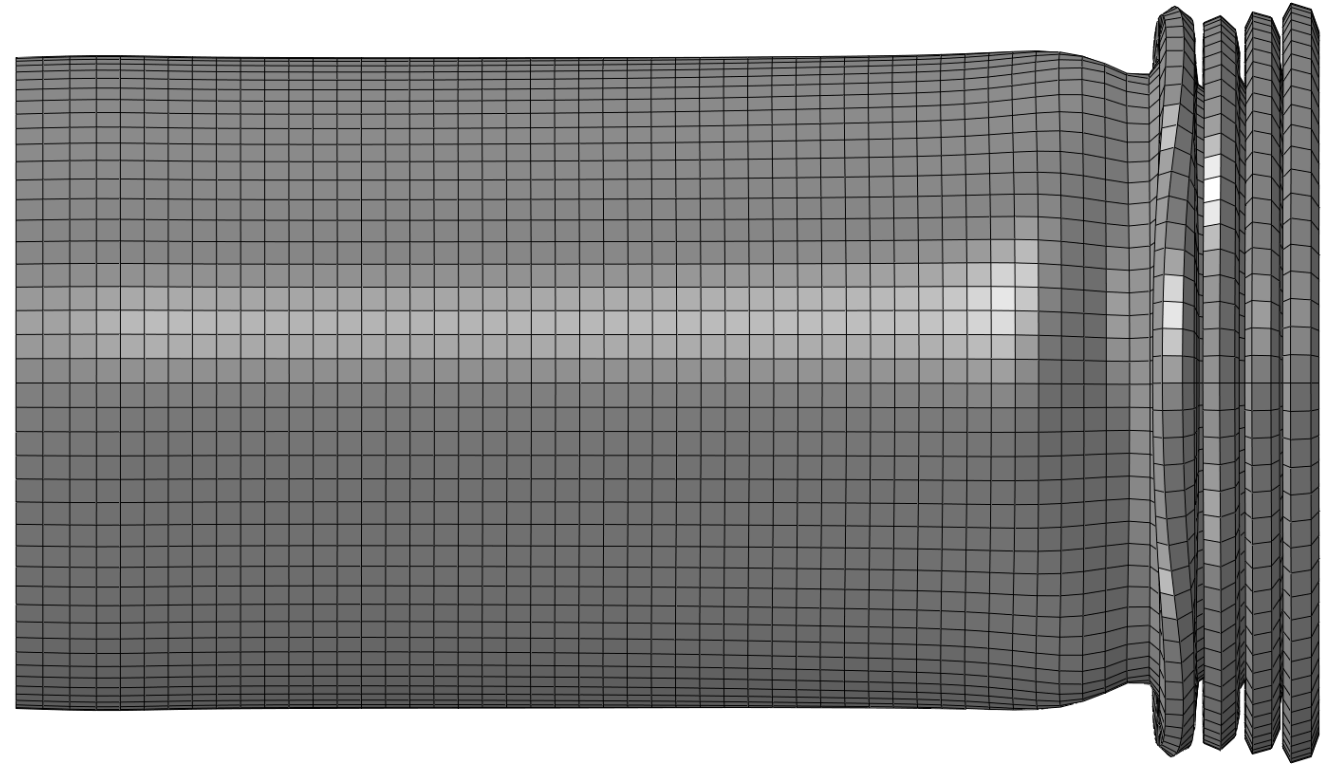
\includegraphics[width=.8\columnwidth, angle=90]{./twt_circ.png}
  \caption{Finite element crushing simulation of circular tube after formation of four folds.}
  \label{fig:twt_circ}
\end{figure}

\begin{figure}[htpb]
  \centering
   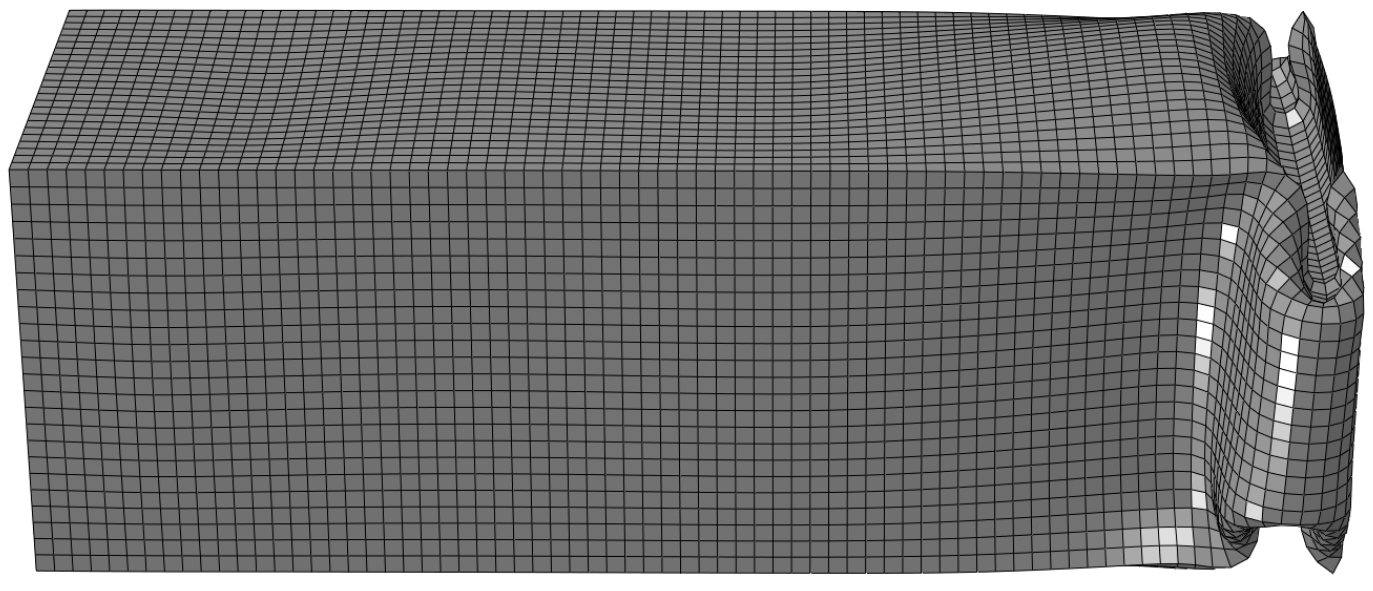
\includegraphics[width=\columnwidth, angle=90.3]{./sq_1fold.png}
  \caption{Finite element crushing simulation of square tube after formation of the first fold.}
  \label{fig:twt_sq}
\end{figure}

\subsubsection{Post-process}

\label{sec:postprocess}
The techniques used for obtaining the force-displacement curves and, consequently, average and peak force values, also have a noteworthy effect on the final results. After the completion of each simulation, a Python script automatically opens the results file and retrieves the unfiltered force-displacement data for the analysis. Later, this data undergoes a SAE 600 filter \cite{J211} as recommended by the literature \citep{Huanglibro}.

For the acquisition of the peak force, it is found that the unfiltered data predicts with a significantly higher accuracy the values provided by \cref{eq:pmax2}, with discrepancies reduced from 27.6\% for the filtered value to 2.2\% for the unfiltered. \Cref{img:fd_unf-filt} shows both response curves for the baseline circular design.

\begin{figure}[htpb]
  \centering
   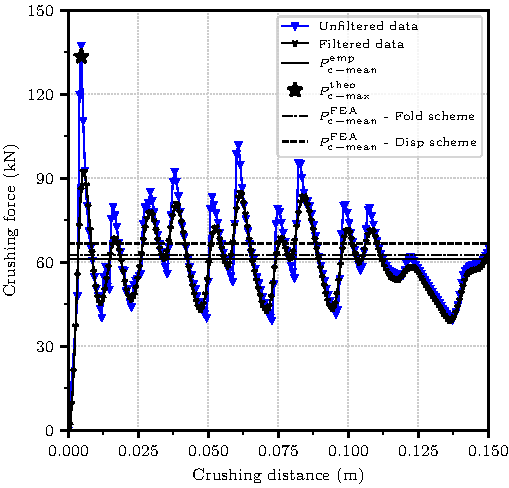
\includegraphics[width=1\columnwidth]{./fd-processing.pdf}
  \caption{.}
  \label{img:fd_unf-filt}
\end{figure}

Moreover, the calculation of $P^{\mathrm{FEA}}_{\mathrm{mean}}$ is performed by two different methods. Initially, the average force is determined by the numerical integration of the area under the curve until a certain crushing distance is reached. However, this entails considering the initial buckling force and not calculating the average force for an integer number of folds, which increases the error and variability of the studied metric. Thus, another post-processing scheme is developed in which $P^{\mathrm{FEA}}_{\mathrm{mean}}$ is averaged for a specified number of full folds  (four full folds are selected for these calculations), increasing the robustness of the post-process and reducing noise for the studied metric. \Cref{img:fd_unf-filt} also offers a graphic depiction of the result for both aforementioned schemes, showing how the displacement scheme overestimates the analytical result for $P^{\mathrm{}}_{\mathrm{mean}}$. 

% Data acquisition \& Filters

% Number of folds retrieved vs crushing distance (imgs with shadowed area considered)

\section{Results}

\subsection{Numerical uncertainties}

\subsubsection{Surrogate performance}



% \textbf{Kriging}

% \cref{fig:surr_stats-krig}

% \begin{figure}[htpb]
% \centering
% \begin{subfigure}[b]{.6\columnwidth}
%   \centering
%   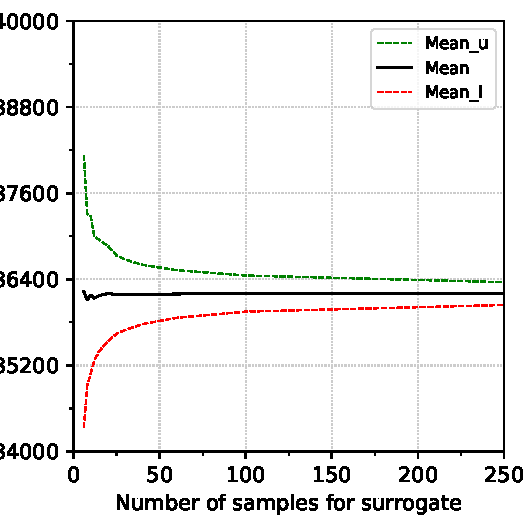
\includegraphics[width=\columnwidth]{./surr_stats_mean-krig.pdf}
%   \caption{Evolution of mean value for $P^{\mathrm{emp}}_{\mathrm{mean}}$ with number of samples used.}
%   \label{fig:surr_stats_mean-krig}
% \end{subfigure}
% ~\\[3pt]
% \begin{subfigure}[b]{.6\columnwidth}
%   \centering
%   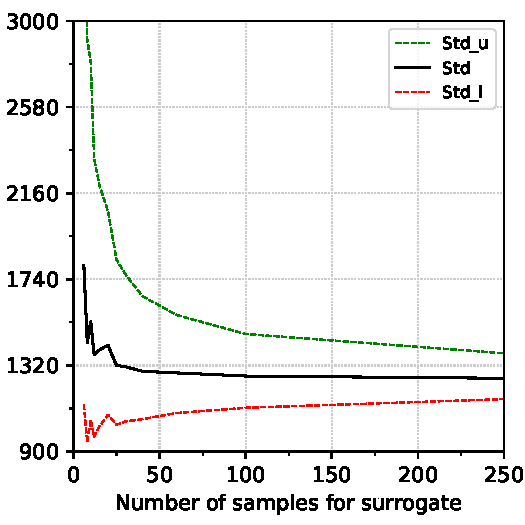
\includegraphics[width=\columnwidth]{./surr_stats_std-krig.pdf}
%   \caption{Evolution of standard deviation for $P^{\mathrm{emp}}_{\mathrm{mean}}$ with number of samples used.}
%   \label{fig:surr_stats_std-krig}
% \end{subfigure}
% \caption{Evolution of statistical moments for $P^{\mathrm{emp}}_{\mathrm{mean}}$ with number of samples used for the Kriging metamodel.}
% \label{fig:surr_stats-krig}
% \end{figure}

% \begin{table*}[!htpb]
% \begin{center}
% % \small
% \begin{tabular}[t]{lrrrrrr} \toprule
% Samples &	Pmean &	Pmean-95CI	& \%95CI	& Std-dev &	Std-dev-95CI	& \%95CI\\\midrule
% 6	 & 66.15 & 	17.07 & 	25.80 & 	8.13 & 	14.87	 & 182.84\\
% 8	 & 65.59 & 	10.75 & 	16.39 & 	6.43 & 	8.84	 & 137.41\\
% 10	 & 65.91 & 	9.86	 & 14.96 & 	6.89 & 	7.84	 & 113.78\\
% 12	 & 65.70 & 	7.78	 & 11.84 & 	6.12 & 	6.06 & 	98.95\\
% 15	 & 65.87 & 	6.95	 & 10.55 & 	6.27 & 	5.30 & 	84.50\\
% 20	 & 66.01 & 	6.00	 & 9.09	 & 6.41	 & 4.49 & 	70.01\\
% 30	 & 65.92 & 	4.39	 & 6.66	 & 5.88	 & 3.22 & 	54.79\\
% 40	 & 65.93 & 	3.73	 & 5.66	 & 5.83	 & 2.71 & 	46.49\\
% 60	 & 65.96 & 	2.99	 & 4.53	 & 5.78	 & 2.15 & 	37.20\\
% 80	 & 65.96 & 	2.52	 & 3.83	 & 5.67	 & 1.81 & 	31.90\\
% 100	 & 65.98 & 	2.27	 & 3.43	 & 5.71 & 1.62 & 	28.37\\
% 250	 & 65.98 & 	1.41	 & 2.14	 & 5.66	 & 1.00 & 	17.69\\
% \bottomrule
% \end{tabular}
% \captionsetup{justification=centering}
% \caption{Krig Metamodel. COV=5.}
% \label{tab:krig}
% \end{center}
% \end{table*}


% \textbf{PRS}

% \cref{fig:surr_stats-pol}

% \begin{figure}[htpb]
% \centering
% \begin{subfigure}[b]{.6\columnwidth}
%   \centering
%   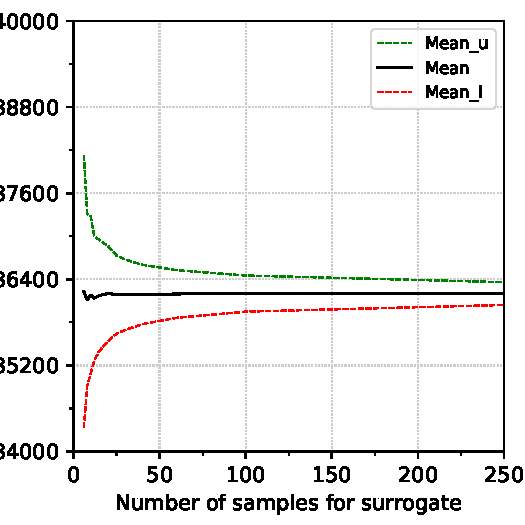
\includegraphics[width=\columnwidth]{./surr_stats_mean-pol.pdf}
%   \caption{Evolution of mean value for $P^{\mathrm{emp}}_{\mathrm{mean}}$ with number of samples used.}
%   \label{fig:surr_stats_mean-pol}
% \end{subfigure}
% ~\\[3pt]
% \begin{subfigure}[b]{.6\columnwidth}
%   \centering
%   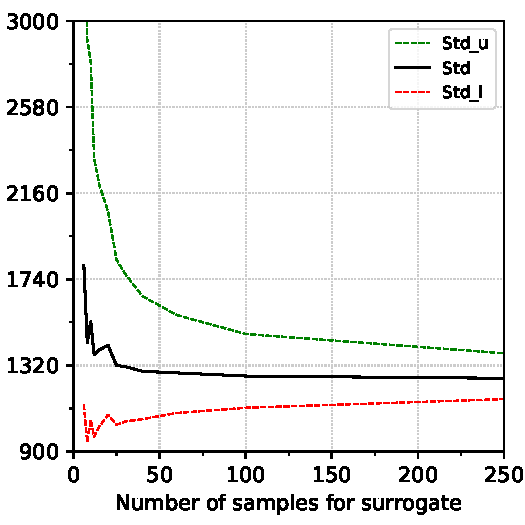
\includegraphics[width=\columnwidth]{./surr_stats_std-pol.pdf}
%   \caption{Evolution of standard deviation for $P^{\mathrm{emp}}_{\mathrm{mean}}$ with number of samples used.}
%   \label{fig:surr_stats_std-pol}
% \end{subfigure}
% \caption{Evolution of statistical moments for $P^{\mathrm{emp}}_{\mathrm{mean}}$ with number of samples used for the Polynomial metamodel.}
% \label{fig:surr_stats-pol}
% \end{figure}


% \textbf{MLS}

% \cref{fig:surr_stats-mls}

% \begin{figure}[htpb]
% \centering
% \begin{subfigure}[b]{.6\columnwidth}
%   \centering
%   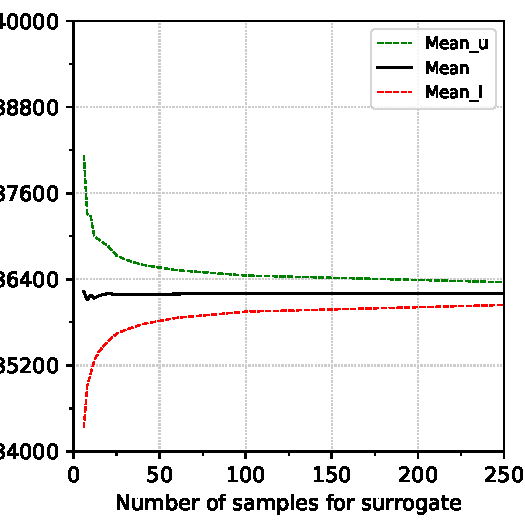
\includegraphics[width=\columnwidth]{./surr_stats_mean-mls.pdf}
%   \caption{Evolution of mean value for $P^{\mathrm{emp}}_{\mathrm{mean}}$ with number of samples used.}
%   \label{fig:surr_stats_mean-mls}
% \end{subfigure}
% ~\\[3pt]
% \begin{subfigure}[b]{.6\columnwidth}
%   \centering
%   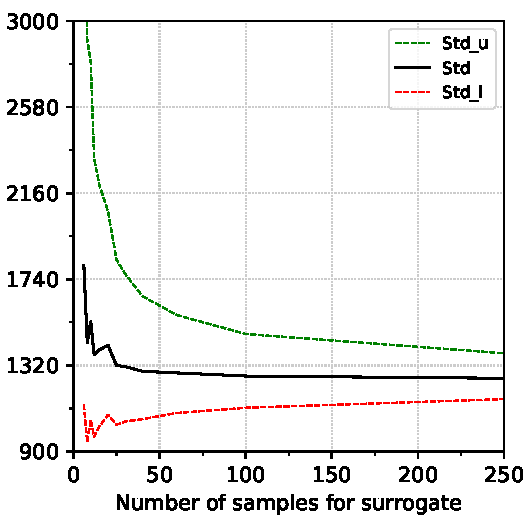
\includegraphics[width=\columnwidth]{./surr_stats_std-mls.pdf}
%   \caption{Evolution of standard deviation for $P^{\mathrm{emp}}_{\mathrm{mean}}$ with number of samples used.}
%   \label{fig:surr_stats_std-mls}
% \end{subfigure}
% \caption{Evolution of statistical moments for $P^{\mathrm{emp}}_{\mathrm{mean}}$ with number of samples used for the Moving Least Squares metamodel.}
% \label{fig:surr_stats-mls}
% \end{figure}

% \textbf{MARS}

To analyze the performance of the surrogate models used and the number of samples required to accurately capture the values and trends of the metrics studied, different comparisons are run both with the analytical formulas and the finite element simulations. The results hereunder presented correspond to the circular tube with geometrical uncertainties (see \cref{tab:vars_circ}) with a $\mathrm{COV} = 5\%$, while the metrics are $P^{\mathrm{emp}}_{\mathrm{c{\text -}mean}}$, $P^{\mathrm{FEA}}_{\mathrm{c{\text -}mean}}$, $P^{\mathrm{theo}}_{\mathrm{c{\text -}max}}$, and $P^{\mathrm{FEA}}_{\mathrm{c{\text -}max}}$.  

First, all four metamodels are compared in terms of $R^2$ and the mean absolute error (MAE) with and without a 10-fold cross-validation scheme. Results from \cref{tab:all_surr}, retrieved from a sampling of 60 models, show that the kriging metamodel outperforms the others for the analytical formulas, not only because of the $R^2 = 1$ inherent to Gaussian processes, but also for the reduced values of the MAE in both $P^{\mathrm{emp}}_{\mathrm{c{\text -}mean}}$ and $P^{\mathrm{theo}}_{\mathrm{c{\text -}max}}$. In the case of $P^{\mathrm{emp}}_{\mathrm{c{\text -}mean}}$, kriging's error is two magnitude orders smaller than that from other surrogates, while for $P^{\mathrm{theo}}_{\mathrm{c{\text -}max}}$ is one magnitude order smaller than MARS and within the same order as the MLS and polynomial metamodels. However, it is important to note than MAE values, even after cross-validation, are less than 1\% of the average value of the metrics, and $R^2 \geq 0.999$ for all four metamodels. Thus, and besides the superior approximation provided by kriging, all four metamodels can be deemed acceptable for accurately predicting $P^{\mathrm{emp}}_{\mathrm{c{\text -}mean}}$ and $P^{\mathrm{theo}}_{\mathrm{c{\text -}max}}$ with the considered number of samples.

Next, a similar procedure is performed but substituting the analytical formulas by the numerical responses $P^{\mathrm{FEA}}_{\mathrm{c{\text -}mean}}$ and $P^{\mathrm{FEA}}_{\mathrm{c{\text -}max}}$. A review of the results for the simulation data in \cref{tab:all_surr} now reveals that the worst fit is provided by kriging, which yields MAE values considerably higher than those from its counterparts. In this case, the MARS metamodel with $2^{\mathrm{nd}}$-order base functions obtains a higher $R^2$ and the lowest MAE value of all four metamodels. 

It is important to note than for this latter case, the metamodel has to accurately estimate the values at the sampling points as well as filtering-out the high-frequency noise from FEA's, which kriging fails to do as it is required to pass through all the sampling points provided. The other three metamodels overcome this on account of having an $R^2 < 1$ but better predicting the value of the function outside the sampling points. Equivalent tests as the one here described were carried out with different uncertainty parameters, COV's, and number of samples, all leading to similar conclusions in terms of surrogate performance. From within the three, and in view of the previous results, the MARS metamodel is selected as the surrogate model for the rest of the investigation. 

\begin{table}[!htpb]
\begin{center}
\footnotesize
\begin{tabular}[t]{llccccc} \toprule
& & \multicolumn{2}{c}{$P^{\mathrm{}}_{\mathrm{c{\text -}mean}}$} & &\multicolumn{2}{c}{$P^{\mathrm{}}_{\mathrm{c{\text -}max}}$} \\\cmidrule{3-4}\cmidrule{6-7}
\multicolumn{2}{c}{Model}  & $R^2$ & MAE (kN) & & $R^2$ & MAE (kN) \\\midrule
\multirow{4}{*}{Analyt.} & Krig & 1.000  & 	\num{5.302e-5} & &	1.000 & 	\num{2.758e-05}\\
& MARS & $\geq 0.999$  & 	\num{5.558e-03} & &	$\geq 0.999$ & 	\num{9.847e-04}\\
& MLS & $\geq 0.999$  & 	\num{1.385e-03} & &	$\geq 0.999$ & 	\num{2.497e-05}\\
& Pol-q & $\geq 0.999$  & 	\num{2.494e-03} & &	$\geq 0.999$ & 	\num{2.406e-05}\\\midrule
\multirow{4}{*}{Simul.} & Krig & -  & 	1.770 & &	- & 	1.405\\
& MARS & 0.985  & 	0.652 & &	0.997 & 	0.897\\
& MLS & 0.952  & 	0.736 & &	0.987 & 	0.904\\
& Pol-q & 0.934 & 	1.065 & &	0.986 & 	0.963\\
\bottomrule
\end{tabular}
\captionsetup{justification=centering}
\caption{Comparison of metamodel performance for $P^{\mathrm{emp}}_{\mathrm{c{\text -}mean}}$, $P^{\mathrm{theo}}_{\mathrm{c{\text -}max}}$, $P^{\mathrm{FEA}}_{\mathrm{c{\text -}mean}}$, and $P^{\mathrm{FEA}}_{\mathrm{c{\text -}max}}$ of a circular tube with geometrical uncertainties ($\mathrm{COV} = 5$, 60 samples). Mean absolute error (MAE) results correspond to values with 10-fold cross-validation.}
\label{tab:all_surr}
\end{center}
\end{table}

Moreover, \cref{tab:mars} presents the evolution of $\mathrm{E}\left[P^{\mathrm{emp}}_{\mathrm{c{\text -}mean}}\right]$ and $\sigma \left[P^{\mathrm{emp}}_{\mathrm{c{\text -}mean}}\right]$ with their 95\% confidence intervals (CI) as the number of samples used for the metamodel construction is increased. The results, also depicted in \cref{fig:surr_stats_mean-mars,fig:surr_stats_std-mars}, show considerable noise for the predicted values of mean and standard deviation when the number of samples is below 30 or 40, with excessively large 95\% CI ranges. Moreover, the software is not able to provide data for $\mathrm{E}\left[P^{\mathrm{theo}}_{\mathrm{c{\text -}max}}\right]$ and	$\sigma\left[P^{\mathrm{theo}}_{\mathrm{c{\text -}max}}\right]$ when the number of samples is below 12 as the number of points is deemed too low. However, as the number of points selected goes over 50, the average values stabilize whith only small fluctuations observed; while the 95\% CI tightens around the predicted value and is only slowly decreased after this point. Thus, and also considering the trade-off between accuracy and computational efficiency, the selected number of samples for the MARS metamodels used is that of 60.

\begin{table*}[!htpb]
\begin{center}
% \small
\begin{tabular}[t]{lrrrr} \toprule
%  &  \multicolumn{2}{c}{Fold-scheme} &  \multicolumn{2}{c}{Disp-scheme} \\\cmidrule{2-5}
% El. size (mm) & Elements & $P^{\mathrm{FEA}}_{\mathrm{mean}}$   (kN)   &    $P^{\mathrm{FEA}}_{\mathrm{max}}$ (kN) & Comp. time (hh:mm)  \\\midrule
Samples &	$\mathrm{E}\left[P^{\mathrm{emp}}_{\mathrm{c{\text -}mean}}\right] \pm 95\% \mathrm{CI}$ &	$\sigma\left[P^{\mathrm{emp}}_{\mathrm{c{\text -}mean}}\right] \pm 95\% \mathrm{CI}$	&	$\mathrm{E}\left[P^{\mathrm{theo}}_{\mathrm{c{\text -}max}}\right] \pm 95\% \mathrm{CI}$ &	$\sigma\left[P^{\mathrm{theo}}_{\mathrm{c{\text -}max}}\right] \pm 95\% \mathrm{CI}$ \\\midrule
6	& $\SI{66,62 \pm	7,77}{}  $ &	$\SI{7,40 \pm 6,76}{}$ &  - & - \\
8	& $\SI{66,01 \pm	4,86}{} $  &	$\SI{5,81 \pm 3,99}{}$ &  - & - \\
10	& $\SI{66,18 \pm	4,25}{}  $ &	$\SI{5,94 \pm 3,38}{}$ &  - & - \\
12	& $\SI{66,03 \pm	3,45}{} $  &	$\SI{5,43 \pm 2,69}{}$ & $\SI{134,25 \pm 5,77}{}$ &	$\SI{9,08 \pm 4,49}{}$ \\
15	& $\SI{66,12 \pm	3,18}{}  $ &	$\SI{5,75 \pm 2,43}{}$ & $\SI{134,41 \pm 5,38}{}$ &	$\SI{9,71 \pm 4,10}{}$ \\
20	& $\SI{66,19 \pm	2,84}{} $  &	$\SI{6,07 \pm 2,13}{}$ & $\SI{134,48 \pm 4,96}{}$ &	$\SI{10,61\pm 3,71}{}$ \\
30	& $\SI{66,02 \pm	2,09}{}  $ &	$\SI{5,59 \pm 1,53}{}$ & $\SI{134,18 \pm 3,62}{}$ &	$\SI{9,71 \pm 2,66}{}$ \\
40	& $\SI{66,01 \pm	1,81}{} $  &	$\SI{5,66 \pm 1,32}{}$ & $\SI{134,15 \pm 3,14}{}$ &	$\SI{9,82 \pm 2,28}{}$ \\
60	& $\SI{65,91 \pm	1,50}{}  $ &	$\SI{5,79 \pm 1,08}{}$ & $\SI{134,16 \pm 2,54}{}$ &	$\SI{9,84 \pm 1,83}{}$ \\
80	& $\SI{65,95 \pm	1,26}{} $  &	$\SI{5,68 \pm 0,91}{}$ & $\SI{134,12 \pm 2,13}{}$ &	$\SI{9,56 \pm 1,52}{}$ \\
100	& $\SI{66,01 \pm	1,12}{}  $ &	$\SI{5,63 \pm 0,80}{}$ & $\SI{134,18 \pm 1,93}{}$ &	$\SI{9,70 \pm 1,38}{}$ \\
250	& $\SI{65,98 \pm	0,71}{} $  &	$\SI{5,67 \pm 0,50}{}$ & $\SI{134,13 \pm 1,20}{}$ &	$\SI{9,67 \pm 0,86}{}$ \\
\bottomrule
\end{tabular}
\captionsetup{justification=centering}
\caption{Evolution of MARS metamodel estimation for the mean and standard deviation values of $P^{\mathrm{emp}}_{\mathrm{c{\text -}mean}}$ and $P^{\mathrm{theo}}_{\mathrm{c{\text -}max}}$ and their 95\% confidence intervals (CI) of a circular tube with geometrical uncertainties ($\mathrm{COV} = 5$).}
\label{tab:mars}
\end{center}
\end{table*}


\begin{figure}[htpb]
\centering
\begin{subfigure}[b]{1.0\columnwidth}
  \centering
   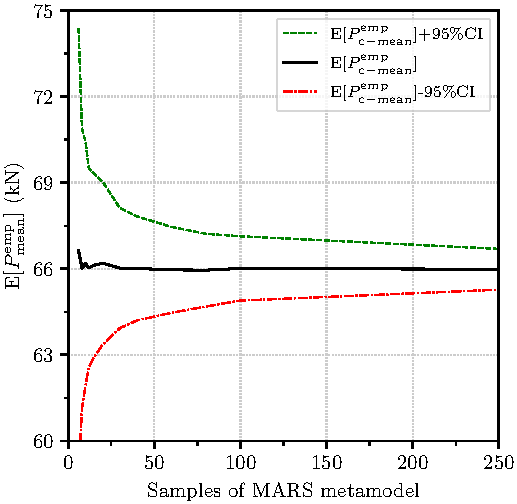
\includegraphics[width=.85\columnwidth]{./surr_stats_mean.pdf}
  \caption{Evolution of mean value for $P^{\mathrm{emp}}_{\mathrm{c{\text -}mean}}$ with number of samples used.}
  \label{fig:surr_stats_mean-mars}
\end{subfigure}
~\\[3pt]
\begin{subfigure}[b]{1.0\columnwidth}
  \centering
   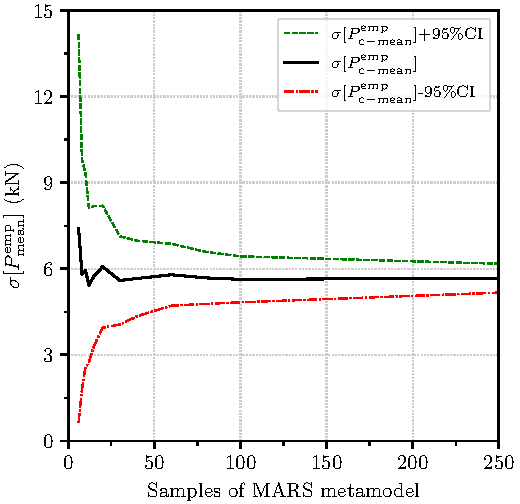
\includegraphics[width=.85\columnwidth]{./surr_stats_std.pdf}
  \caption{Evolution of standard deviation for $P^{\mathrm{emp}}_{\mathrm{c{\text -}mean}}$ with number of samples used.}
  \label{fig:surr_stats_std-mars}
\end{subfigure}
\caption{Evolution of statistical moments for $P^{\mathrm{emp}}_{\mathrm{c{\text -}mean}}$ with number of samples used for the MARS metamodel.}
\label{fig:surr_stats-mars}
\end{figure}

\subsubsection{Numerical noise}

Numerical noise in FEA is also a source of error in uncertainty propagation. Following a similar approach to that of \citet{gilkeson_dealing_2014}, this investigation will also attempt to quantify the oscillation frequency and standard deviation of the numerical responses. The baseline circular tube is chosen, allowing the thickness to vary between $1.5 \leq t_\mathrm{c} \leq 2.5$, while disregarding variations in the diameter as this would slightly change the mesh definition and introduce further sources of noise.

As a benchmark for the FEA, the analytical formulas are first used for ${P}^{\mathrm{emp}}_{\mathrm{c{\text -}mean}}$ and ${P}^{\mathrm{theo}}_{\mathrm{c{\text -}max}}$. Then, an homologous procedure is repeated with ${P}^{\mathrm{FEA}}_{\mathrm{c{\text -}mean}}$ and ${P}^{\mathrm{FEA}}_{\mathrm{c{\text -}max}}$, with the former being retrieved through both schemes described in \cref{sec:postprocess}. \Cref{fig:Pmean_evolution2,fig:Pmax_evolution2} offer the comparison between the analytical and numerical responses as the plate thickness progressively increases, easily distinguishing the results from the simulation by their fluctuations around the analytical values.

Moreover, these results are normalized with respect to the tube's thickness, dividing the results by a constant and the tube's thickness raised to a power, which leads to $\overline{P}^{\mathrm{}}_{\mathrm{c{\text -}mean}} = {P}^{\mathrm{}}_{\mathrm{c{\text -}mean}} / \left(\beta_1 t_{\mathrm{c}}^{1.68}\right)$ and $\overline{P}^{\mathrm{}}_{\mathrm{c{\text -}max}} = {P}^{\mathrm{}}_{\mathrm{c{\text -}max}} / \left(\beta_2 t_{\mathrm{c}}^{2}\right)$, where $\beta_1$ and $\beta_2$ are the constants that normalize \cref{eq:pmean_emp,eq:pmax2}. These techniques allow the characterization of noise as represented in \cref{fig:Pmean_evolution_normalized,fig:Pmax_evolution_normalized}. 


% \Cref{tab:num_noise,fig:Pmean_evolution2,fig:Pmean_evolution_normalized,fig:Pmax_evolution2,fig:Pmax_evolution_normalized}

% $\overline{P}^{\mathrm{}}_{\mathrm{mean}}$ = ${P}^{\mathrm{}}_{\mathrm{mean}} / \left(\beta_1 t_{\mathrm{c}}^{1.68}\right)$ and $\overline{P}^{\mathrm{}}_{\mathrm{max}}$ = ${P}^{\mathrm{}}_{\mathrm{max}} / \left(\beta_2 t_{\mathrm{c}}^{2}\right)$

\begin{figure}[htpb]
  \centering
   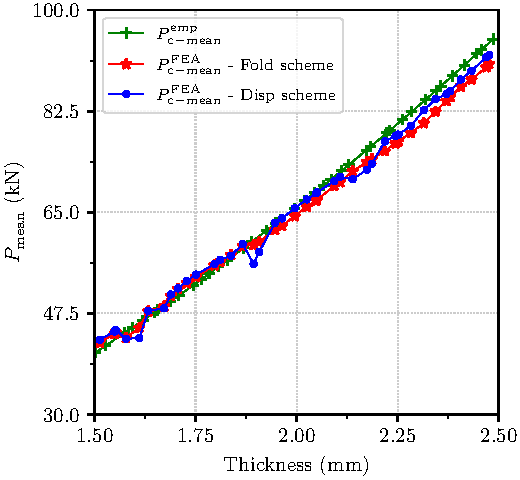
\includegraphics[width=.9\columnwidth]{./Pmean_evolution.pdf}
  \caption{Evolution of $P^{\mathrm{emp}}_{\mathrm{c{\text -}mean}}$ and $P^{\mathrm{FEA}}_{\mathrm{c{\text -}mean}}$ due to thickness variation. Results from \cref{eq:pmean_emp} and FEA with the two post-process schemes. Results based on 40 samples.}
  \label{fig:Pmean_evolution2}
\end{figure}

\begin{figure}[htpb]
  \centering
   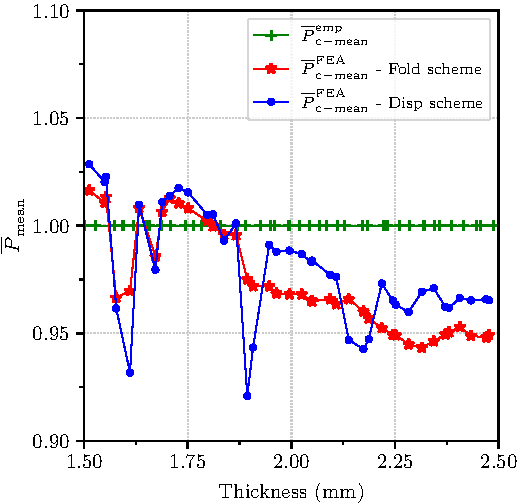
\includegraphics[width=.9\columnwidth]{./Pmean_evolution_normalized.pdf}
   \caption{Evolution of normalized $\overline{P}^{\mathrm{emp}}_{\mathrm{c{\text -}mean}}$ and $\overline{P}^{\mathrm{FEA}}_{\mathrm{c{\text -}mean}}$ due to thickness variation. Results from \cref{eq:pmean_emp} and FEA with the two postprocess schemes. Results based on 40 samples.}
  \label{fig:Pmean_evolution_normalized}
\end{figure}

\begin{figure}[htpb]  
  \centering
   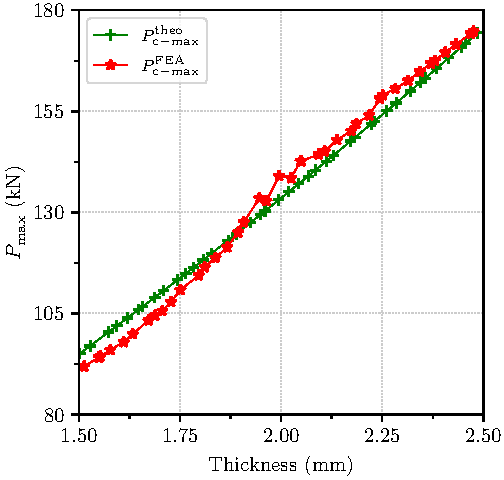
\includegraphics[width=.9\columnwidth]{./Pmax_evolution.pdf}
  \caption{Evolution of $P^{\mathrm{theo}}_{\mathrm{c{\text -}max}}$ and $P^{\mathrm{FEA}}_{\mathrm{c{\text -}max}}$ due to thickness variation. Results from \cref{eq:pmax2} and FEA. Results based on 40 samples.}
  \label{fig:Pmax_evolution2}
\end{figure}

\begin{figure}[htpb]
  \centering
   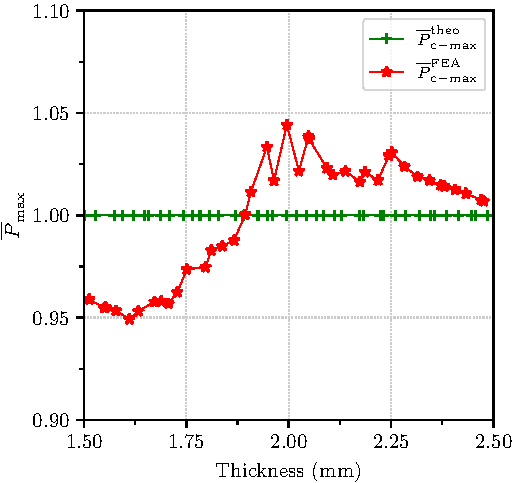
\includegraphics[width=.9\columnwidth]{./Pmax_evolution_normalized.pdf}
  \caption{Evolution of normalized $\overline{P}^{\mathrm{theo}}_{\mathrm{c{\text -}max}}$ and $\overline{P}^{\mathrm{FEA}}_{\mathrm{c{\text -}max}}$ due to thickness variation. Results from \cref{eq:pmax2} and FEA. Results based on 40 samples.}
  \label{fig:Pmax_evolution_normalized}
\end{figure}


The results for the analytical values in \cref{tab:num_noise} show a perfect fit, yielding a constant value of $\overline{P}^{\mathrm{theo}}_{\mathrm{c{\text -}mean}} = \overline{P}^{\mathrm{theo}}_{\mathrm{c{\text -}max}} = 1$ for both metrics, while those from the FEA offer relevant values of noise. When comparing both post-process schemes for obtaining ${P}^{\mathrm{FEA}}_{\mathrm{c{\text -}mean}}$, the fold scheme has a slight advantage with better resemblance with the empirical results, a smaller standard deviation, and nearly half the oscillation frequency. This high oscillation frequency can constitute a hindering factor during the construction of most surrogate models, specially true for Gaussian processes which are required to pass through all the sampling points. Moreover, the breadth of $A_{3 \sigma}$ (the area of the 95\% CI) is just over 6.5\% for the fold-scheme, while the integration of ${P}^{\mathrm{FEA}}_{\mathrm{c{\text -}mean}}$ by means of a constant displacement leads to an $A_{3 \sigma}$ of nearly 8\%. Thus, the fold-scheme is selected for the rest of this investigation.

The performance of $\overline{P}^{\mathrm{FEA}}_{\mathrm{c{\text -}max}}$ is also evaluated, yielding an oscillation frequency of 40\%. Furthermore, the average fit of this metric within the studied thickness range is nearly that of the analytical results, although a closer look at \cref{fig:Pmax_evolution_normalized} reveals how values are slightly under-predicted for thickness below 1.85 mm, and over-predicted after that value. However, the area of the 95\% CI for this metric is under 9\%, considered an acceptable value given the non-linear and dynamic nature of these simulations.


\begin{table*}[!htpb]
\begin{center}
% \footnotesize
\begin{tabular}[t]{lrrrrr} \toprule
%  &  \multicolumn{2}{c}{Analytical} & \multicolumn{3}{c}{Simulation}  \\\cmidrule{2-3}\cmidrule{4-6}
Metric & $\overline{P}^{\mathrm{emp}}_{\mathrm{c{\text -}mean}}$     & $\overline{P}^{\mathrm{theo}}_{\mathrm{c{\text -}max}}$   &    $\overline{P}^{\mathrm{FEA}}_{\mathrm{c{\text -}mean}}$ (folds)   & $\overline{P}^{\mathrm{FEA}}_{\mathrm{c{\text -}mean}}$ (disp)   &    $\overline{P}^{\mathrm{FEA}}_{\mathrm{c{\text -}max}}$   \\\midrule
Mean (kN)  &  1.000 & 1.000 & 0.979  & 0.974 & 0.999  \\
Std (kN) &  0.0 & 0.0 & 0.0219 &  0.0264 & 0.0297   \\\midrule
Osc. freq (\%) &  0.0 & 0.0 &  32.5 & 60.0 & 40.0  \\
$A_{\sigma}$ (\%) & 0.0 & 0.0 &  2.19 & 2.64 & 2.97   \\
$A_{3 \sigma}$ (\%) & 0.0 & 0.0 &  6.57 & 7.95 & 8.92   \\
\bottomrule
\end{tabular}
\captionsetup{justification=centering}
\caption{Statistical moments and numerical noise quantification \citep{gilkeson_dealing_2014} for normalized $\overline{P}^{\mathrm{}}_{\mathrm{c{\text -}mean}}$ and $\overline{P}^{\mathrm{}}_{\mathrm{c{\text -}max}}$ with analytical results and FEA after both post-process schemes. Results based on 40 samples.}
\label{tab:num_noise}
\end{center}
\end{table*}

\subsection{Circular tube}

In this section, the propagation of geometrical, material, and impact uncertainties on the axially-loaded circular tube is presented. %Results are obtained through the analytical propagation of the formulas, ...

\subsubsection{Geometrical uncertainties}  

First, the diameter and plate thickness of the tube are assumed to be defined by a normal distribution with three different coefficients of variation. The propagation of variables is to be performed with both combined, studying its effect on the mean and peak crushing loads.

In the results presented in \cref{tab:UQ_circ1}, it is first seen that the mean value for $P^{\mathrm{emp}}_{\mathrm{c{\text -}mean}}$ resulting from the statistical propagation and the surrogate model is matched to the second decimal place, although minor discrepancies in the standard deviation are observed overshooting the value by 1\% to 3\%. This is considered an acceptable error for the purposes here intended, although it could be reduced by increasing the sampling size.

Among the three metrics studied, $P^{\mathrm{theo}}_{\mathrm{c{\text -}max}}$ has the smallest COV resulting values, while the results from $P^{\mathrm{emp}}_{\mathrm{c{\text -}mean}}$ and  $P^{\mathrm{theo}}_{\mathrm{c{\text -}mean}}$ are fairly similar. Overall, the COV of the resulting metric after the combination of two uncertainty sources is increased less than 50\% of the original COV value. 

Uncertainty propagation is also performed with the two metrics retrieved from the FEA. When comparing the expected values for $P^{\mathrm{emp}}_{\mathrm{c{\text -}mean}}$ and $P^{\mathrm{FEA}}_{\mathrm{c{\text -}mean}}$, the difference is less than 0.1\%, while the variation between analytical and numerical peak crushing loads is around 1\%. The propagation based on numerical simulations also yields similar COVs than the analytical formulas, which are progressively reduced for both the mean and peak crushing forces as the COV of the variables is increased. 

\begin{table*}[!htpb]
\begin{center}
% \footnotesize
\begin{tabular}[t]{llrrrr} \toprule
 & &  &  \multicolumn{3}{c}{Standard deviation}  \\\cmidrule{4-6}
&  & Mean       &    COV = 2 \%  &  COV = 5 \%      &    COV = 10 \%  \\\midrule
\multirow{2}{*}{Variables} & $D$ (mm) &  80.00 &  1.60 & 4.00 & 8.00   \\
& $t_\mathrm{c}$ (mm) &  2.00 & 0.04 & 0.10 & 0.20 \\ \midrule
\multirow{1}{*}{Analytical (stat)} & $P^{\mathrm{emp}}_{\mathrm{c{\text -}mean}}$ (kN) &  65.91 & 2.25 (3.41\%) & 5.64 (8.56\%) &  11.29 (17.13\%)   \\\midrule
% & $P^{\mathrm{theo}}_{\mathrm{c{\text -}mean}}$ (kN) & 63.50  &  (\%) &  (\%) &  (\%)  \\
% & $P^{\mathrm{theo}}_{\mathrm{c{\text -}max}}$ (kN) & 134.03  &  (\%) &  (\%) &  (\%) ) \\ \midrule
\multirow{3}{*}{Analytical (surr)} & $P^{\mathrm{emp}}_{\mathrm{c{\text -}mean}}$ (kN) &  65.91 &  2.32 (3.52\%) & 5.78 (8.77 \%) & 11.55 (17.52 \%)  \\
& $P^{\mathrm{theo}}_{\mathrm{c{\text -}mean}}$ (kN) & 63.50  & 2.16 (3.40\%) & 5.39 (8.49\%) & 10.76 (16.94\%) \\
& $P^{\mathrm{theo}}_{\mathrm{c{\text -}max}}$ (kN) & 134.16  & 4.00 (2.92\%) & 9.84 (7.34\%) & 19.83 (14.61\%) \\ \midrule
\multirow{2}{*}{Simulation} & $P^{\mathrm{FEA}}_{\mathrm{c{\text -}mean}}$ (kN) &  65.85 & 2.33 (3.54\%) & 5.33 (8.09\%) & 9.98 (15.16\%)  \\
& $P^{\mathrm{FEA}}_{\mathrm{c{\text -}max}}$ (kN) &  135.76  & 4.13 (3.04\%) & 9.42 (6.94\%) & 18.31 (13.49\%) \\
% $\nu$  &  0.33 & - & - & - \\
% $\rho$ $\mathrm{kg/m^3}$ & 2700  & - & - & - \\
\bottomrule
\end{tabular}
\captionsetup{justification=centering}
\caption{Statistical moments for the geometrical design parameters and studied analytical metrics for the circular tube with three different COV. Values in brackets correspond to resulting COV for the metrics. Results based on 60 samples.}
\label{tab:UQ_circ1}
\end{center}
\end{table*}

\subsubsection{Material uncertainties}

The uncertainty propagation procedure is repeated with material variability and presented in \cref{tab:UQ_circ2}, obtaining similar discrepancies in the expected value of the metrics between the numerical and analytical methods. However, since  $P^{\mathrm{emp}}_{\mathrm{c{\text -}mean}}$ and  $P^{\mathrm{theo}}_{\mathrm{c{\text -}mean}}$ from \cref{eq:pmean_emp,eq:pmean_theo} are independent of $E$, the resulting standard deviations and COVs obtained from the analytical and metamodel propagation match almost perfectly the COV from the $\sigma_0$ variable. In the case of $P^{\mathrm{theo}}_{\mathrm{c{\text -}max}}$, which is influenced by both variables, the resulting variance is around 15\% lower than that of a single variable. 

Finally, the results from FEAs also show differences from mean values under 0.1\% and 1\% for average and peak crushing loads respectively. The propagation based on numerical simulations also yields lower COVs than the analytical formulas, which can be up to half of those for mean crushing forces and around 15\% for the $P^{\mathrm{}}_{\mathrm{c{\text -}max}}$.

% Effect of E and yield stress \Cref{tab:UQ_circ2}.

\begin{table*}[!htpb]
\begin{center}
% \footnotesize
\begin{tabular}[t]{llrrrr} \toprule
 & &  &  \multicolumn{3}{c}{Standard deviation}  \\\cmidrule{4-6}
&  & Mean       &    COV = 2 \%  &  COV = 5 \%      &    COV = 10 \%  \\\midrule
\multirow{2}{*}{Variables} & E (GPa)  &  73.10 &  1.462 & 3.655 & 7.310   \\
 & $\sigma_0$ (MPa) &  280.00 & 5.60 & 14.00 & 28.00 \\ \midrule
\multirow{1}{*}{Analytical (stat)} & $P^{\mathrm{emp}}_{\mathrm{c{\text -}mean}}$ (kN) &  65.91  & 1.32 (2.00\%) &  3.30 (5.00\%) & 6.59 (10.00\%) \\\midrule
% & $P^{\mathrm{theo}}_{\mathrm{c{\text -}mean}}$ (kN) & 63.50  & 1.27 (2.00\%) & 3.17 (4.99\%) & 6.35 (10.00\%) \\
% & $P^{\mathrm{theo}}_{\mathrm{c{\text -}max}}$ (kN) & 134.04  & 2.21 (1.64\%) & 5.52 (4.12\%) & 11.09 (8.27\%) \\ \midrule
\multirow{3}{*}{Analytical (surr)} & $P^{\mathrm{emp}}_{\mathrm{c{\text -}mean}}$ (kN) &  65.92  & 1.32 (2.00\%) &  3.29 (4.99\%) & 6.59 (10.00\%) \\
& $P^{\mathrm{theo}}_{\mathrm{c{\text -}mean}}$ (kN) & 63.50  & 1.27 (2.00\%) & 3.17 (4.99\%) & 6.35 (10.00\%) \\
& $P^{\mathrm{theo}}_{\mathrm{c{\text -}max}}$ (kN) & 134.04  & 2.21 (1.64\%) & 5.52 (4.12\%) & 11.09 (8.27\%) \\ \midrule
\multirow{2}{*}{Simulation} & $P^{\mathrm{FEA}}_{\mathrm{c{\text -}mean}}$ (kN) &  65.89 & 0.60 (0.91\%) & 1.52 (2.31\%) & 2.96 (4.49\%)  \\
& $P^{\mathrm{FEA}}_{\mathrm{c{\text -}max}}$ (kN) &  135.76  & 1.91 (1.41\%) & 4.04 (2.98\%) & 10.31 (7.59\%) \\
% $\nu$  &  0.33 & - & - & - \\
% $\rho$ $\mathrm{kg/m^3}$ & 2700  & - & - & - \\ 
\bottomrule
\end{tabular}
\captionsetup{justification=centering}
\caption{Statistical moments for the geometrical design parameters and studied analytical metrics for the circular tube with three different COV. Values in brackets correspond to resulting COV for the metrics. Results based on 60 samples.}
\label{tab:UQ_circ2}
\end{center}
\end{table*}

\subsubsection{Impact conditions uncertainties}

The uncertainty quantification for circular tubes finalizes with variations in impact conditions. This is only studied here with the metamodels from numerical simulations rather than using the analytical formulas. The results in \cref{tab:UQ_circ3} show how the expected value of $P^{\mathrm{FEA}}_{\mathrm{c{\text -}mean}}$ decreases around 1.5\% with respect to that obtained from the previous uncertainty propagation. The evolution of the standard deviations and COVs, however, offer a peculiar behavior in which the COV is increased from 2\% in the variables to 2.65\% in the resulting metric, while it decreases from 10\% to 6.82\% in the latest case. This can be explained by a higher sensitivity of the responses when varying close to the average value, while being of a lesser effect as the variables take values further from the average.

On the other hand, the evolution of the standard deviations of $P^{\mathrm{FEA}}_{\mathrm{c{\text -}max}}$ presents the opposite behavior, increasing the COV of the resulting metrics as the standard deviation of the variables increases. A similar under-prediction in the average value of $P^{\mathrm{FEA}}_{\mathrm{c{\text -}max}}$ is also found, with an estimation 16\% lower than the expected force. 

% DOE angle / velocity

\begin{table*}[!htpb]
\begin{center}
% \footnotesize
\begin{tabular}[t]{llrrrr} \toprule
 & &  &  \multicolumn{3}{c}{Standard deviation}  \\\cmidrule{4-6}
&  & Mean       &    COV = 2 \%  &  COV = 5 \%      &    COV = 10 \%  \\\midrule
\multirow{2}{*}{Variables} & V (m/s)  &  0.2 &  0.004 & 0.01 & 0.02   \\
 & $\theta_{\mathrm{imp}}$ (Degrees) &  90 & 1.8 & 4.5 & 9.0 \\ \midrule
% \multirow{3}{*}{Num responses} & $P^{\mathrm{emp}}_{\mathrm{c{\text -}mean}}$ (kN) &  61.23  & (\%) & ( \%) & ( \%) \\
% & $P^{\mathrm{theo}}_{\mathrm{c{\text -}mean}}$ (kN) &   & (\%) & ( \%) & ( \%) \\
% & $P^{\mathrm{}}_{\mathrm{c{\text -}max}}$ (kN) & 133.51  & (\%) & ( \%) & ( \%) \\ \midrule
\multirow{2}{*}{Simulation} & $P^{\mathrm{FEA}}_{\mathrm{c{\text -}mean}}$ (kN) &  64.94 & 1.72 (2.65\%) & 3.09 (4.75\%) & 4.42 (6.82\%)  \\
& $P^{\mathrm{FEA}}_{\mathrm{c{\text -}max}}$ (kN) &  113.83  & 15.38 (13.51\%) & 35.81 (31.46\%) & 84.75 (74.45\%) \\
% $\nu$  &  0.33 & - & - & - \\
% $\rho$ $\mathrm{kg/m^3}$ & 2700  & - & - & - \\
\bottomrule
\end{tabular}
\captionsetup{justification=centering}
\caption{Statistical moments for the geometrical design parameters and studied analytical metrics for the circular tube with three different COV. Values in brackets correspond to resulting COV for the metrics. Results based on 60 samples.}
\label{tab:UQ_circ3}
\end{center}
\end{table*}

\subsection{Square tube}

Now, the homologous uncertainty propagation procedures used with the circular tube are applied to the square-sectioned component.
\subsubsection{Geometrical uncertainties}

A first comparison of the mean predictions for $P^{\mathrm{}}_{\mathrm{s{\text -}mean}}$ shows almost equal values between the numerical and analytical results, with the those from the FEA being 1\% lower than the empirical formula. Moreover, the usage of surrogate models induces a similar error in the calculation of the standard deviations of $P^{\mathrm{emp}}_{\mathrm{s{\text -}mean}}$ and  $P^{\mathrm{theo}}_{\mathrm{s{\text -}mean}}$ as with the circular tube, overpredicting the moment by 0.7\% to 1\%. This is kept consistent for the three COV studied and both mean crushing force formulas.

In the case of $P^{\mathrm{}}_{\mathrm{s{\text -}max}}$, the difference between the average values is more significant than with the circular tube with the analytical surrogate yielding a value 8.5\% higher than the numerical simulation, although this can be attributed to a uniform disparity between the results of both predictions. When looking at the standard deviations, however, it is clear that dispersion from the metamodel from FEAs is notably lower, leading to COVs in the resulting metrics up to 55\% lower than the ones provided from the analytical formulas. 

% Effect of thickness, edge length. \Cref{tab:analytical_sq}.

\begin{table*}[!htpb]
\begin{center}
% \footnotesize
\begin{tabular}[t]{llrrrr} \toprule
 & &  &  \multicolumn{3}{c}{Standard deviation}  \\\cmidrule{4-6}
&  & Mean       &    COV = 2 \%  &  COV = 5 \%      &    COV = 10 \%  \\\midrule
\multirow{2}{*}{Variables} &  $C$ (mm) &  70.90 &  1.418 & 3.545 & 7.090   \\
& $t_\mathrm{s}$ (mm) &  1.77 & 0.0354 & 0.0885 & 0.177 \\ \midrule
\multirow{2}{*}{Analytical (stat)} & $P^{\mathrm{emp}}_{\mathrm{s{\text -}mean}}$ (kN) & 33.65  & 1.14 (3.40\%) & 2.86 (8.50\%) & 5.73 (17.02\%)   \\
& $P^{\mathrm{theo}}_{\mathrm{s{\text -}mean}}$ (kN) & 29.04  & 0.99 (3.40\%) & 2.47 (8.50\%) & 4.94 (17.02\%)  \\\midrule
% & $P^{\mathrm{theo}}_{\mathrm{s{\text -}max}}$ (kN) &   &  (\%) &  (\%) &  (\%)  \\ \midrule
\multirow{3}{*}{Analytical (surr)} & $P^{\mathrm{emp}}_{\mathrm{s{\text -}mean}}$ (kN) & 33.66  & 1.16 (3.44\%) & 2.89 (8.59\%) & 5.77 (17.14\%)    \\
& $P^{\mathrm{theo}}_{\mathrm{s{\text -}mean}}$ (kN) & 29.04  & 1.00 (3.44\%) & 2.50 (8.61\%) & 4.99 (17.18\%)   \\
& $P^{\mathrm{theo}}_{\mathrm{s{\text -}max}}$ (kN) & 139.94  & 9.91 (7.08\%) & 24.93 (17.81\%) & 51.21 (36.59\%) \\ \midrule
\multirow{2}{*}{Simulation} & $P^{\mathrm{FEA}}_{\mathrm{s{\text -}mean}}$ (kN) & 33.32  & 2.02 (6.06\%) & 4.02 (12.06\%) & 6.01 (18.03\%)  \\
& $P^{\mathrm{FEA}}_{\mathrm{s{\text -}max}}$ (kN) & 127.91 & 3.86 (3.02\%) & 9.04 (7.07\%) & 20.70 (16.18\%) \\
% $\nu$  &  0.33 & - & - & - \\
% $\rho$ $\mathrm{kg/m^3}$ & 2700  & - & - & - \\
\bottomrule
\end{tabular}
\captionsetup{justification=centering}
\caption{Statistical moments for the material parameters and studied analytical metrics for the square tube with three different COV. Values in brackets correspond to resulting COV for the metrics. Results based on 60 samples.}
\label{tab:analytical_sq}
\end{center}
\end{table*}

\subsubsection{Material uncertainties}

The study of material uncertainties for the square tube reveals a similar behavior as its examination with the circular counterpart. Both analytical equations for $P^{\mathrm{}}_{\mathrm{s{\text -}mean}}$ are independent of the Young's modulus, thus leading to matching COVs between $\sigma_0$ and $P^{\mathrm{}}_{\mathrm{s{\text -}mean}}$ as shown in \cref{tab:UQ_sqc2}. However, $P^{\mathrm{theo}}_{\mathrm{s{\text -}max}}$ does consider both variables for its calculation, increasing the COV of the results by less than 50\% of the variables' COV.

The analysis of the simulation results, in which both variables affect the result metrics, offers similar mean values as those stemming from geometrical uncertainties, where the average crushing force almost matches $P^{\mathrm{emp}}_{\mathrm{s{\text -}mean}}$ and $P^{\mathrm{FEA}}_{\mathrm{s{\text -}max}}$ is 8.5\% lower than the prediction from the formula. For the standard deviations and their respective COVs, the metamodel from FEAs performs better in the estimation of the average crushing load, reducing the COV by approxiamtely 50\% from the analytical solutions. In the case of the peak crushing force, however, the standard deviations and COVs are higher when computed with numerical simulation as a consequence of being metric with hogher fluctuations and more prone to numerical noise.

% Effect of E and yield stress. \Cref{tab:UQ_sqc2}.

\begin{table*}[!htpb]
\begin{center}
% \footnotesize
\begin{tabular}[t]{llrrrr} \toprule
 & &  &  \multicolumn{3}{c}{Standard deviation}  \\\cmidrule{4-6}
&  & Mean       &    COV = 2 \%  &  COV = 5 \%      &    COV = 10 \%  \\\midrule
\multirow{2}{*}{Variables} & E (GPa)  &  73.10 &  1.462 & 3.655 & 7.310   \\
 & $\sigma_0$ (MPa) &  280.00 & 5.60 & 14.00 & 28.00 \\ \midrule
\multirow{2}{*}{Analytical (stat)} & $P^{\mathrm{emp}}_{\mathrm{s{\text -}mean}}$ (kN) & 33.65  & 0.67 (2.00\%) & 1.68 (5.00\%) & 3.37 (10.00\%)   \\
& $P^{\mathrm{theo}}_{\mathrm{s{\text -}mean}}$ (kN) & 29.04  & 0.58 (2.00\%) & 1.45 (5.00\%) & 2.90 (10.00\%)  \\\midrule
% & $P^{\mathrm{theo}}_{\mathrm{s{\text -}max}}$ (kN) &   &  (\%) &  (\%) &  (\%)  \\ \midrule
\multirow{3}{*}{Analytical (surr)} & $P^{\mathrm{emp}}_{\mathrm{s{\text -}mean}}$ (kN) & 33.65  & 0.67 (2.00\%) & 1.68 (5.00\%) & 3.36 (9.99\%)    \\
& $P^{\mathrm{theo}}_{\mathrm{s{\text -}mean}}$ (kN) & 29.04  & 0.58 (2.00\%) & 1.45 (5.00\%) & 2.90 (10.00\%)   \\
& $P^{\mathrm{theo}}_{\mathrm{s{\text -}max}}$ (kN) & 139.94  & 3.86 (2.76\%) & 9.72 (6.95\%) & 19.80 (14.15\%) \\ \midrule
\multirow{2}{*}{Simulation} & $P^{\mathrm{FEA}}_{\mathrm{s{\text -}mean}}$ (kN) & 33.32 & 0.28 (0.84\%) & 1.11 (3.33\%) & 1.67 (5.01\%)   \\
& $P^{\mathrm{FEA}}_{\mathrm{s{\text -}max}}$ (kN) & 127.91 & 4.78 (3.74\%) & 12.09 (9.45\%) & 19.01 (14.86\%)  \\
% $\nu$  &  0.33 & - & - & - \\
% $\rho$ $\mathrm{kg/m^3}$ & 2700  & - & - & - \\ 
\bottomrule
\end{tabular}
\captionsetup{justification=centering}
\caption{Statistical moments for the geometrical design parameters and studied analytical metrics for the circular tube with three different COV. Values in brackets correspond to resulting COV for the metrics. Results based on 60 samples.}
\label{tab:UQ_sqc2}
\end{center}
\end{table*}

\subsubsection{Impact conditions uncertainties}

The last of the uncertainty propagation results is carried out by using the impact angle and velocity as variables. These results, obtained only from numerical simulations and presented in \cref{tab:UQ_sq3}, manifest mean values 3.5\% higher for $P^{\mathrm{FEA}}_{\mathrm{s{\text -}mean}}$ and around 15\% lower for $P^{\mathrm{FEA}}_{\mathrm{s{\text -}max}}$. As with the circular tube, it becomes apparent that the effect of impact angle variations leads to a significant consequence on the peak force results. Still, in the case of the average value, this seems to be of a minor effect, with COVs for $P^{\mathrm{FEA}}_{\mathrm{s{\text -}mean}}$ being reduced by as much as to a fourth of the variables' COV.

To further understand the effect of the impact angle on the tube's response, \cref{fig:fd-angle} contains the force-displacement graphs for the square baseline tube where the impact angle is gradually decreased from 90 to 80 degrees. In the comparison it is easily perceived how by only reducing the angle by 2 degrees, the peak force is decreased from 127.9 kN to 65.2 kN, nearly half of the original value. As the impact angle is further reduced, the $P^{\mathrm{FEA}}_{\mathrm{s{\text -}max}}$ now is lowered at a smaller rate, hitting a values around 50-55 kN when the angle reaches 82 degrees. This significant non-linear behavior of the studied metric explain the values for $P^{\mathrm{FEA}}_{\mathrm{s{\text -}max}}$ obtained in \cref{tab:UQ_sq3}, both in the reduced mean value and the high standard deviations with all three COVs. Per contra, $P^{\mathrm{FEA}}_{\mathrm{s{\text -}mean}}$ suffers an antagonistic comportment to the peak force, as its expected value is increased by 3.5\% and the resulting COV is that of 2.32\% even with a variables' COV of 10\%. In this case, the variations in impact angle which severely affected the peak force at the beginning of the crushing process, do not have a major effect on the rest of the response in terms of average load. In  \cref{fig:fd-angle} it is clearly seen how after the initial 10 mm of crushing the curves all follow a similar trend, and even the lower impact angles can yield higher loads in some parts of the crushing process.
% Effect of impact velocity and impact angle. \Cref{tab:UQ_sq3}.

% Graph with comparison f-d for different angles

\begin{table*}[!htpb]
\begin{center}
% \footnotesize
\begin{tabular}[t]{llrrrr} \toprule
 & &  &  \multicolumn{3}{c}{Standard deviation}  \\\cmidrule{4-6}
&  & Mean       &    COV = 2 \%  &  COV = 5 \%      &    COV = 10 \%  \\\midrule
\multirow{2}{*}{Variables} & V (m/s)  &  0.2 &  0.004 & 0.01 & 0.02   \\
 & $\theta_{\mathrm{imp}}$ (Degrees) &  90 & 1.8 & 4.5 & 9.0 \\ \midrule
\multirow{2}{*}{Simulation} & $P^{\mathrm{FEA}}_{\mathrm{s{\text -}mean}}$ (kN) & 34.50  & 0.43 (1.25\%) & 0.44 (1.28\%) & 0.80 (2.32\%)  \\
& $P^{\mathrm{FEA}}_{\mathrm{s{\text -}max}}$ (kN) & 108.72  & 12.01 (11.05\%) & 17.04 (15.67\%) & 58.55 (53.85\%)  \\
% $\nu$  &  0.33 & - & - & - \\
% $\rho$ $\mathrm{kg/m^3}$ & 2700  & - & - & - \\
\bottomrule
\end{tabular}
\captionsetup{justification=centering}
\caption{Statistical moments for the geometrical design parameters and studied analytical metrics for the square tube with three different COV. Values in brackets correspond to resulting COV for the metrics. Results based on 60 samples.}
\label{tab:UQ_sq3}
\end{center}
\end{table*}

\begin{figure}[htpb]
  \centering
   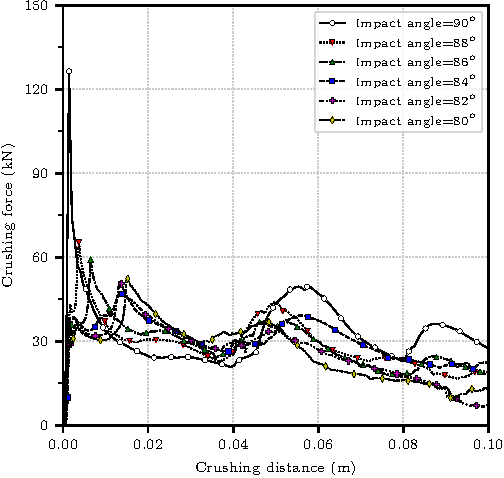
\includegraphics[width=\columnwidth]{./fd-angle.pdf}
  \caption{Force - displacement curves of baseline square tube crushed with different impact angles.}
  \label{fig:fd-angle}
\end{figure}

% \subsection{}
\subsection{Tube comparison}

The tubes' geometries were selected so that both cross-sections have the same solidity ratio, in this case $\phi^c = \phi^s = 0.1$. When this condition is met, the following is also true: 
\begin{equation}
\frac{\eta^c}{\eta^s} = \frac{P^{\mathrm{}}_{\mathrm{c{\text -}mean}}}{P^{\mathrm{}}_{\mathrm{s{\text -}mean}}}    
\end{equation}

This equality, applied to the empirical formulas, which provide the best agreement with the simulations, is nearly achieved with ${\eta_{\mathrm{emp}}^c}/\eta_{\mathrm{emp}}^s=1.81$ and ${P^{\mathrm{emp}}_{\mathrm{c{\text -}mean}}}/{P^{\mathrm{emp}}_{\mathrm{s{\text -}mean}}} = 1.88$, confirming a slight but acceptable error in the predictions.

The efficiency of both configurations is also compared in terms of the energy-absorbing effectiveness factor $\psi$, defined as the ratio between the elastic and plastic strain energy absorbed by a structure, and the energy absorbed in the same volume of material up to failure in tension \citep{hsu2004quasi,jones2005energy,jones2010energy}. This energy-absorbing effectiveness factor can be written as

\begin{equation}
\psi = \frac{\int_0^{\delta_f} P \, \mathrm{d}\delta}{V \int_0^{\epsilon_f} \sigma \mathrm{d}\epsilon} = \frac{P^{\mathrm{}}_{\mathrm{mean}} \delta_f}{\sigma_0 A_c \, L \, \epsilon_f}, 
\label{eq:psi}
\end{equation}
where $P$ is the axial crushing force and $\delta$ the crushing distance, comprised between 0 and the final value $\delta_f$, with $\delta_f \approx 0.75 L$. In the denominator, $V$ represents the volume of material of the specimen, while $\sigma$ is the tensile stress, and $\epsilon$ and $\epsilon_f$ are the uniaxial engineering strain and rupture strain respectively. According to \cref{eq:psi}, the effectiveness factor for the circular tube is $\psi_c = 1.61$, whereas the square tube yields a $\psi_s = 0.83$, leading to this circular section being nearly twice as efficient as the square counterpart.

When looking at the results from the uncertainty propagation of both designs there seem to be some common behaviors, specially in the case of geometric uncertainties. In the simple correlation matrix from \cref{tab:corr_matrix}, it is seen that the plate thickness of the tubes has the greatest effect on both metrics, with coefficents ranging betweem 0.81 and 0.97. The diameter and length have a smaller impact, with a correlation coefficient around 0.2 for average crushing loads and a higher value of approximately 0.55 for the peak force. However, material uncertainties affect both tubes in the opposite manner, as the elastic modulus has the greatest effect on the metrics for the square section, while flow stress values reach correlation values over 0.93 with the circular tube. Finally, correlation values for the impact variables are mostly below 0.1 and even take negative values, in concordance with the results previosly presented in \cref{tab:UQ_circ3,tab:UQ_sq3}. 

\begin{table}[!htpb]
\begin{center}
% \small
\begin{tabular}[t]{lccccc} \toprule
& \multicolumn{2}{c}{$P^{\mathrm{FEA}}_{\mathrm{mean}}$} & &\multicolumn{2}{c}{$P^{\mathrm{FEA}}_{\mathrm{max}}$}  \\\cmidrule{2-3}\cmidrule{5-6}
Variable  & Circ & Sq & & Circ & Sq \\\midrule
$D$ / $C$ & 0.218 & 0.227 & & 0.558	 & 0.541 \\
$t_\mathrm{c}$ / $t_\mathrm{s}$  & 0.978 & 0.813	 & & 0.939	 & 0.934 \\\midrule
$E$ & 0.302 & 0.860	 & & 0.263	 & 0.687 \\
$\sigma_0$ & 0.952 & -0.062 & & 0.937	 & 0.599 \\\midrule
V & 0.856 & 0.019 & & 0.032	 & -0.264 \\
$\theta_{\mathrm{imp}}$ & 0.218 & 0.071	 & & -0.071	 & -0.045\\
\bottomrule
\end{tabular}
\captionsetup{justification=centering}
\caption{ Simple correlation matrix between variables and response metrics for the circular and square tubes. Results obtained for the MARS surrogate from the numerical simulations, with 60 sampling points and COV = 2\%}
\label{tab:corr_matrix}
\end{center}
\end{table}

\section{Conclusions}

In the research described in this paper, the analytical and numerical crashworthiness uncertainty quantification of two aluminum thin-walled energy absorbers is performed, considering the average and peak crushing loads as metrics. Three different approaches are followed: a statistical error propagation of the analytical formulas, the UQ from a surrogate model from the formulas, and from a surrogate model built from finite element simulations. The following conclusions can be withdrawn:

\begin{itemize}
    \item The use of surrogate models for the uncertainty quantification of the analytical formulas here studied yields similar mean values as with statistical propagation, although the standard deviation is overshot between 1\% and 3\%.
    \item The performance comparison between the four metamodels studied shows that MARS outperforms the others when stemming from numerical simulations, while offering similar $R^2$ to the other in the case of analytical formulas. A study on sample size returns acceptable error values when 60 or more samples are used.
    \item Numerical noise from the simulations displays an oscillation frequency below 40\% for both metrics, while $A_{3 \sigma}$ is approximately 6.5\% and 9\% for the average and peak crushing loads respectively.
    \item The calculation of the average crushing force from the force-displacement curves is proved to be more robust when integrating a fixed number of fold rather than a fixed crushing distance. Results offer a better agreement with the analytical formulas and less noise in the average load metric.
    \item The use of properly adjusted numerical simulations can accurately match the results from the analytical formulas when calculating the statistical moments during the UQ process. The circular tube offers a sightly better agreement with the formulas than the square counterpart.
    \item Both tube configurations are similarly affected from the geometric uncertainties, where plate thickness is more influential on the results than diameter or edge length. In the case of material uncertainties, the elastic modulus is the most influential variable for the square section, whereas the equivalent flow stress has the highest correlation with the metrics from the circular tube.
    \item Uncertainties in the impact conditions can only be studied via metamodels constructed from numerical simulations. The average crushing load can be retrieved with an acceptable accuracy, where the square section proves to be more robust than the circular. Peak load values rapidly decrease when the impact angle varies from a perfect axial collision, leading to reduced mean values and high standard deviations after the error propagation.
\end{itemize}

% \clearpage
% \newpage
\section*{Acknowledgements}
The research leading to these results has received funding from the Spanish Goverment (\textit{Ministerio de Econom\'{\i}a y Competitividad}) under grant agreement DPI2016-76934-R. The authors fully acknowledge the support received. The authors also wish to acknowledge the help and advice provided by Dr. Luis Ramirez. 

% \section*{Planning}

% Analytical formulas, circular and square, theoretical and empirical (Pm, Pmax, Strain-rate) 

% - Propagate error analytically. Thickness, E, edge-radius, impact velocity

% - Propagate error numerically (Dakota)

% Numerical (FEM)

% - Propagate error numerically (Abq + Dakota)

% ---

% Results:

% - Analytical vs. numerical vs. FEA mean values / std deviations

% - Quantify metamodel and FEA noise-error


% \clearpage
\bibliography{./UQrefs.bib}

\clearpage

\onecolumn
\appendix
\section{Analytical propagation of uncertainty}
\label{sec:app1}
The analytical uncertainty propagation of the formulas presented in \cref{sec:intro} is now described. Considering the formula from \cref{eq:pmean_emp} as means of example\footnote{An homologous procedure is also used with \cref{eq:pmean_emp_sq2,eq:pmean_theo_sq}}, it is first divided into a coefficient and two simpler functions as
\begin{align}
P^{\mathrm{emp}}_{\mathrm{c{\text -}mean}} = 72.3 & (D / t_\mathrm{c})^{0.32} \sigma_{0} \; {t_\mathrm{c}}^2 / {4} = \alpha_1 g(D) \; h(t_\mathrm{c}), \\   
\mathrm{where} & \nonumber \\
 \alpha_1 &= 72.3 \sigma_0 /4, \\
 g(D) &= D ^{0.32}, \; \; \mathrm{and}\\ 
 h(t_\mathrm{c}) &= t_\mathrm{c}^{1.68}
\end{align}

With the formula divided, now the expected value $E[\,]$ and variance $V[\,]$ can be calculated using the following properties of the statistical moments:
\begin{align}
E[\alpha_1 g(D) \; h(t_\mathrm{c})] &= \alpha_1  E[g(D)] \; E[h(t_\mathrm{c})] \label{eq:e1}\\% = \alpha_1  g(E[x]) \; h(E[y]) \\
V[\alpha_1 g(D) \; h(t_\mathrm{c})] &= \alpha_1^2  ( E^2[g(D)] \; V[h(t_\mathrm{c})] + V[g(D)] \; E^2[h(t_\mathrm{c})] + V[g(D)] \; V[h(t_\mathrm{c})]) \label{eq:v1}
\end{align}
where
\begin{align}
E[g(D)] &= {\left.{g(D)}\right|_{E[D]}} \label{eq:e2}\\
E[h(t_\mathrm{c})] &= \left.{h(t_\mathrm{c})}\right|_{E[t_\mathrm{c}]} \label{eq:e3}
\end{align}
% \begin{align}
% E[\alpha_1 g(D) \; h(t_\mathrm{c})] &= \alpha_1  E[g(D)] \; E[h(t_\mathrm{c})] \\% = \alpha_1  g(E[x]) \; h(E[y]) \\
% V[\alpha_1 g(D) \; h(t_\mathrm{c})] &= \alpha_1^2  ( E^2[g(D)] \; V[h(t_\mathrm{c})]  \\
% & + V[g(D)] \; E^2[h(t_\mathrm{c})] + V[g(D)] \; V[h(t_\mathrm{c})])
% \end{align}

Moreover, to calculate the variance of $g(D)$ and $h(t_\mathrm{c})$, the following approximations using second-order Taylor expansion series are used
\begin{align}
% E[\alpha_1 g(x) \; h(y)] &= \alpha_1  E[g(x)] \; E[h(y)] \\% = \alpha_1  g(E[x]) \; h(E[y]) \\
V[g(D)] &= {\left( \left.\frac{d g(D)}{d D}\right|_{E[D]} \right)}^2 V[D] + \frac{1}{2} {\left( \left.\frac{d^2 g(D)}{d D^2}\right|_{E[D]} \right)}^2 V^2[D] \label{eq:v2}\\%  \frac{d g(x)}{d x} \\
V[h(t_\mathrm{c})] &= {\left( \left.\frac{d h(t_\mathrm{c})}{d t_\mathrm{c}}\right|_{E[t_\mathrm{c}]} \right)}^2 V[t_\mathrm{c}] + \frac{1}{2} {\left( \left.\frac{d^2 h(t_\mathrm{c})}{d t_\mathrm{c}^2}\right|_{E[t_\mathrm{c}]} \right)}^2 V^2[t_\mathrm{c}] \label{eq:v3}
\end{align}
which, after coupling them with \cref{eq:e1,eq:v1} yields

\begin{align}
E[P^{\mathrm{emp}}_{\mathrm{c{\text -}mean}}] &=  E[\alpha_1 g(D) \; h(t_\mathrm{c})] = \alpha_1 {\left( \left.{g(D)}\right|_{E[D]} \right)}  {\left( \left.{h(t_\mathrm{c})}\right|_{E[t_\mathrm{c}]} \right)} \label{eq:ef1}\\
V[P^{\mathrm{emp}}_{\mathrm{c{\text -}mean}}] &=  V[\alpha_1 g(D) \; h(t_\mathrm{c})] =  \alpha_1^2 \left[ {\left( \left.{g(D)}\right|_{E[D]} \right)}^2   {\left( {\left( \left.\frac{d h(t_\mathrm{c})}{d t_\mathrm{c}}\right|_{E[t_\mathrm{c}]} \right)}^2 V[t_\mathrm{c}] + \frac{1}{2} {\left( \left.\frac{d^2 h(t_\mathrm{c})}{d t_\mathrm{c}^2}\right|_{E[t_\mathrm{c}]} \right)}^2 V^2[t_\mathrm{c}] \right)} + \right. \nonumber \\
&+ {\left( \left.{h(t_\mathrm{c})}\right|_{E[t_\mathrm{c}]} \right)}^2   {\left( {\left( \left.\frac{d g(D)}{d D}\right|_{E[D]} \right)}^2 V[D] + \frac{1}{2} {\left( \left.\frac{d^2 g(D)}{d D^2}\right|_{E[D]} \right)}^2 V^2[D] \right)} + \nonumber \\
&+ \left.{\left( {\left( \left.\frac{d h(t_\mathrm{c})}{d t_\mathrm{c}}\right|_{E[t_\mathrm{c}]} \right)}^2 V[t_\mathrm{c}] + \frac{1}{2} {\left( \left.\frac{d^2 h(t_\mathrm{c})}{d t_\mathrm{c}^2}\right|_{E[t_\mathrm{c}]} \right)}^2 V^2[t_\mathrm{c}] \right)}  {\left( {\left( \left.\frac{d g(D)}{d D}\right|_{E[D]} \right)}^2 V[D] + \frac{1}{2} {\left( \left.\frac{d^2 g(D)}{d D^2}\right|_{E[D]} \right)}^2 V^2[D] \right)} \right] \label{eq:vf1}
\end{align}

As a last step, if \cref{eq:ef1,eq:vf1} are particularized for $D \sim \mathcal{N}(\mu_\mathrm{D},\,\sigma_\mathrm{D}^{2})\,$ and $t_\mathrm{c} \sim \mathcal{N}(\mu_\mathrm{t_\mathrm{c}},\,\sigma_\mathrm{t_\mathrm{c}}^{2})\,,$ the following expressions are obtained:

\begin{align}
E[P^{\mathrm{emp}}_{\mathrm{c{\text -}mean}}] &=  \alpha_1 g(\mu_\mathrm{D}) \; h(\mu_\mathrm{t_\mathrm{c}}) \label{eq:ef2}\\
V[P^{\mathrm{emp}}_{\mathrm{c{\text -}mean}}] &=  \alpha_1^2 \left[ { {g(\mu_\mathrm{D})} }^2   {\left( {h'(\mu_\mathrm{t_\mathrm{c}})}^2 \sigma_\mathrm{t_\mathrm{c}}^{2} + \frac{1}{2} {{h''(\mu_\mathrm{t_\mathrm{c}})}^2 \sigma_\mathrm{t_\mathrm{c}}^{4}}  \right)} +  { {h(\mu_\mathrm{t_\mathrm{c}})} }^2   {\left( {g'(\mu_\mathrm{D})}^2 \sigma_\mathrm{D}^{2} + \frac{1}{2} {{g''(\mu_\mathrm{D})}^2 \sigma_\mathrm{D}^{4}}  \right)}   \right. + \nonumber \\
&+ \left.{\left( {h'(\mu_\mathrm{t_\mathrm{c}})}^2 \sigma_\mathrm{t_\mathrm{c}}^{2} + \frac{1}{2} {{h''(\mu_\mathrm{t_\mathrm{c}})}^2 \sigma_\mathrm{t_\mathrm{c}}^{4}}  \right)} {\left( {g'(\mu_\mathrm{D})}^2 \sigma_\mathrm{D}^{2} + \frac{1}{2} {{g''(\mu_\mathrm{D})}^2 \sigma_\mathrm{D}^{4}}  \right)} \right]\label{eq:vf2}
\end{align}

\end{document}

